%
% You may wish to use some of the following options of the iitthesis
% package:
%
% fullpageDraft      avoid the margins necessary for proper binding and
%   just view or print a draft.
% beforeDefense      make the personal acknowledgements invisible;
%   use this to print the copies you submit initially to the grad school
%   for sending to the opponent panel, i.e. thesis readers (who shouldn't
%   see those parts). For the final submission, after having successfully
%   defended - drop this option.
% noabbrevs          avoid generation of a notation & abbreviations list
%
% Additionally, you must specify the degree for which you're writing
% your thesis (MSc/PhD/MArch etc.)
%
\documentclass[PhD, with-ethics-statement, fullpageDraft, beforeDefense]{misc/iitthesis}


% Definitions of info fields for the thesis - subject, advisor,
% faculty, acknowledgements, etc. etc. The thesis-fields file 
% contains Hebrew text, and should use the UTF-8 character set
% encoding (not iso-8859-8-i or windows codepage 1255).
% This file contains definitions of various fields used
% in various places throughout the thesis (in the title
% pages mostly). Whatever isn't define here has some
% default (and usually irrelevant) text.

\authorEnglish{Christoph Velling}
\authorHebrew{כריסטוף פלינג}

\titleEnglish{Spatio-temporal \\ microbial evolution dynamics}
\titleHebrew{דינמיקה מרחבית־זמנית \\ של אבולוציה מיקרוביאלית}

\disciplineEnglish{Biology}
\disciplineHebrew{ביולוגיה}

\supervisionEnglish{This research was carried out under the supervision of Prof.~Roy Kishony, in the Faculty of Biology.}
\supervisionHebrew{המחקר בוצע בהנחייתו של פרופסור רועי קישוני, בפקולטה לביולוגיה.}

\GregorianDateEnglish{September 2025}
\GregorianDateHebrew{ספטמבר \textenglish{2025}}
\JewishDateEnglish{Tishrei 5786}
\JewishDateHebrew{תשרי התשפ"ו}

%\financialAcknowledgementEnglish{The Technion's funding of this research is hereby acknowledged.}
%\financialAcknowledgementHebrew{הכרת תודה מסורה לטכניון על מימון מחקר זה.}

% \publicationInfoEnglish{%
% %Remove this parenthesized note and the line following it!
% (The grad school guidelines now require that you mention the following regarding publications of your thesis work; but of course, remove this parenthesized note...; you will find the note in the \texttt{thesis-fields.tex} file. The entries for the publication list are BiBTeX bibliography entries, separate from those in the main bibliography: You must place them in \texttt{front/pubinfo.bib}; make sure their labels are distinct from entries in the main bibliography; and order them in the order in which you want them to appear --- they will not be sorted. Note also that the document may need to be processed several times before the list of publications actually appears)

% Some results in this thesis have been published as articles by the author and research collaborators in conferences and journals during the course of the author's doctoral research period, the most up-to-date versions of which being:

% \butcheredbibliography{front/pubinfo.bib}
% }
\ethicsStatementEnglish{%
The research underlying this thesis was conducted honestly, in accordance with the ethical standards customary in academia. This applies, in particular, to the collection, processing and presentation of data, the description of and comparison with previous research work, etc. 
Also, the report on research activities and findings in this work is thorough and honest in accordance with the aforementioned standards.

}

% \publicationInfoHebrew{%
% (התייחסות לפרסומים, שמופיעה להלן, הינה הכרחית לפי תקנות ביה"ס ללימודי מוסמכים; כמובן שיש למחוק את ההערה הזו שבסוגריים... תוכן זה נמצאה בקובץ \textenglish{\texttt{thesis-fields.tex}}. הרשומות לצורך רשימת הפרסומים הינן רשומות \textenglish{BibTeX}, נפרדות מן הרשומות בביבליוגרפיה העיקרית של המסמך: עליך לשים אותן בקובץ \textenglish{\texttt{front/pubinfo.bib}}; הקפיד/י שהתוויות שלהם יהיו שונות מתוויות הרשומות בביליוגרפיה העיקרית. רשום/י אותם בסדר בהם תרצה/י שיופיעו ברשימה --- שכן הן לא ימוינו. כן שים/י לב שייתכן שיהיה צורך להדר את המסמך פעם או פעמיים נוספות עד שהרשימה אכן תופיע כראוי.)

% חלק מן התוצאות בחיבור זה פורסמו כמאמרים מאת המחבר ושותפיו למחקר בכנסים ובכתבי-עת במהלך תקופת מחקר הדוקטורט של המחבר, אשר גרסאותיהם העדכניות ביותר הינן:%

% \begin{otherlanguage}{english}%
% \butcheredbibliography{front/pubinfo.bib}
% \end{otherlanguage}%
% }

\ethicsStatementHebrew{%
המחקר שבבסיס חיבור זה נערך כולו ביושר, ולפי אמות המידה האתיות המקובלות באקדמיה. בפרט אמורים הדברים בפעילויות איסוף הנתונים, עיבודם והצגתם, התייחסות והשוואה למחקרים קודמים וכו', ככל שהיוו חלק מן המחקר. כמו כן, הדיווח על המחקר ותוצאותיו בחיבור זה הוא מלא וישר, לפי אותן אמות מידה.

}
\addbibresource{back/paperpile.bib}
% \thesisbibstyle{trad-alpha}


% Personal acknowledgements (are only used for the post-exam
% version)
\input{front/personal-acks}

% A separate file for the abstract - in English and in Hebrew, so
% you must make sure it's also in the UTF-8 character set encoding.
%
% This file contains the abstract part of your thesis - in English and
% in Hebrew (within \abstractEnglish and \abstractHebrew respectively).
%
% Notes:
% - This file uses the UTF-8 character set encoding for the Hebrew
%   text not to get garbled. Keep it that way.
% - Assuming your thesis is mainly in English, Graduate School 
%   regulations mandate the following lengths for the abstracts:
%
%      Language    Min. Length   Max. Length
%     ---------------------------------------
%      English       200 words     500 words
%      Hebrew        500 words   2,000 words
%
%   so that the Hebrew abstract typically has some content from
%   the English introduction and an overview of the results, not
%   present in the English; it is not just a translation.

\abstractEnglish{

In natural microbial communities, antagonistic interactions among bacterial species, or between bacteria and phages, are important drivers of community evolution and ecological dynamics. These natural environments often involve spatial structure, which could be a key factor for evolutionary processes as well as for expansion dynamics into new spaces, yet it is often neglected in microbial community experimentation and simulations. In this thesis we will present two projects, one experimental one and one modeling a biological system \textit{in-silico}. In the first project, we investigated selection and evolution of antibiotic producers in microdroplets, a microfluidic environment, effectively forming small, distinct environments where direct competition with resistant bacteria is excluded and, therefore, selection for producers can occur. We are able to modify an existing microfluidic system to allow stable production and long-term incubation of microdroplets, containing interacting bacterial communities. We aimed to create a selection mechanism for antibiotic-producing bacteria due to the artificial spatial structure of the microdroplets. In contrast to a well-mixed environment, the benefit of producing an antibiotic is not shared in this case, and therefore, there is a selective advantage for the producing bacteria. However, after an extensive screening of target strains and choosing a producer-target pair, we were not able to grow the producer properly in droplets and could show that the producer does not survive in droplets and does not produce an antibiotic in liquid culture but only on solid growth media. In the second project, we used a simple reaction-diffusion model to study bacteria-phage interactions in a spatially structured environment when phage-sensitive and phage-resistant bacteria are competing for resources. We focus on the impact of resistance and different properties of resistant bacteria. The system exhibits traveling waves, common for such a model and exhibits a steady state moving through space. We show how in such a model phage-resistant bacteria can protect sensitive bacteria through an indirect slowdown of phage migration, in contrast to a simulated well-mixed, chemostat environment where competition with phage-resistant bacteria leads to extinction of phage-sensitive bacteria. Exploring the possible parameter space, we show how phages could potentially overcome this protection mechanism. Lastly, we show that resistant bacteria are necessary to observe this effect and nutrient limitation alone is not sufficient. Together, these studies help shed light on the complex spatio-temporal dynamics of antagonistically interacting microbial species. 

% At this point you write the abstract of your work, in the main language in which it is written (in this template - English). Graduate school regulations require the abstract to constitute an independent whole and be understood to a reader with general knowledge of the field. Use complete sentences and make few or no citations. Do not refer to the main body of the work and do not use uncommon shorthand, symbols and terms unless you have room for explaining them. The English abstract should be between 200 and 500 words long.

% So this should contain a few more paragraphs... we'll fill them using some placeholder text (in Latin):

% \lipsum[10-12]

} % end of English abstract


\abstractHebrew{

% Note that certain commands don't work that well in Hebrew "mode".
% If this happens to you, try wrapping the command within a
% \textenglish{ } - that may (or may not) help.

Add abstract in Hebrew

% כאן יבוא תקציר מורחב בעברית (כאשר שפת החיבור העיקרית היא אנגלית). היקף התקציר יהיה \textenglish{1000-2000} מילים. התקציר יהווה שלמות בפני עצמו ויהיה מובן לקורא בעל ידיעות כלליות בנושא.

% בית הספר ללימודי מוסמכים מנחה מספר הנחיות לגבי התקציר בעברית:
% \begin{itemize}
% \item על התקציר להיכתב במשפטים מקושרים שלמים.
% \item בדרך-כלל אין לציין בתקציר מקורות ספרותיים וציטוטים.
% \item אין להתייחס למספר של פרק, סעיף, נוסחה, ציור או טבלה שבגוף החיבור, ואין להשתמש בקיצורים, סמלים ומונחים לא מקובלים, אלא אם יש בתקציר די מקום לזיהויים.
% \end{itemize}

% לעתים יש בכל-זאת יש צורך לכלול פקודה הכוללת קישור פנימי או חיצוני בתוך התקציר העברי; במצבים כאלו כדאי דרך-כלל לעטוף את הפקודה היוצרת את הקישור בתוך פקודת \textenglish{\texttt{\textbackslash{}textenglish\{\}}} כדי למנוע כל מיני פורענויות בלתי-רצויות, כגון כישלון בהידור קובץ ה-\textenglish{PDF} או שימוש בגופן העברי באופן אשר עלול שלא להנעים לעין. לדוגמה: נניח שיש לנו צורך לצטט מקור ביבליוגרפי. אם נעשה זאת סתם-כך: \textenglish{\texttt{\textbackslash{}cite\{Hoeffding\}}}, נקבל: \cite{Hoeffding}; אם נעטוף את פקודת הציטוט, כך: \textenglish{\texttt{\textbackslash{}textenglish\{\textbackslash{}cite\{Hoeffding\}\}}}, נקבל \textenglish{\cite{Hoeffding}} (כפי שהציטוטים נראים גם בטקסט באנגלית).

% \subsection*{\texthebrew{תת-חלק בתקציר המורחב}}

% תוכן מקוצר לגבי נושא מסוים. התייחסות ל\emph{מושג} מסוים שהחיבור בוחן. וכולי וכולי.


% \subsection*{\texthebrew{נקודה מעניינת לגבי העמודים בעברית}}

% שימו לב כי העמודים בעברית אמורים להיות מיוצרים בסדר ה''הפוך'', הווה אומר העמוד האחרון בקובץ ה-\textenglish{PDF} הוא הכריכה העברית, לפניו השער העברי, ודפי התקציר צריכים להופיע בסדר הפוך (וכן במספור רומי, לפי נהלי הטכניון). כך אם נתבונן במספר שבתחתית עמוד זה \textenglish{---} אשר צריך להיות העמוד הראשון בתקציר-המורחב מבחינת רצף התוכן, והינו העמוד האחרון מבין עמודי התקציר-המורחב אחרון בקובץ ה-\textenglish{PDF} \textenglish{---} נמצא את המספר \textenglish{i} ...

% \newpage

% ... ואילו עמוד זה של התקציר-המורחב בעברית \textenglish{---} שהינו העמוד השני בתקציר-המורחב מבחינת רצף התוכן, ונמצא ראשון בקובץ ה-\textenglish{PDF} \textenglish{---} ממוספר ב-\textenglish{ii}. המטרה במספור בסדר ה"הפוך" היא, שבעת ההדפסה לא יהיה צורך להפוך דפים, לשנות את סדרם וכולי \textenglish{---} רק להדפיס ולכרוך.

 } % end of Hebrew abstract


% Comment this if you do not want a list of abbreviations and acronyms
% (if you have used the noabbrevs option).
% Use this file to create "glossary entries" for abbreviations and acronyms,
% and other notation. The entries defined here don't necessarily have to be 
% used in the thesis (but then you have to decide whether or not to display
% the unused entries).

% For this file to compile (and the example text in the main/prelims.tex file),
% the package glossaries-extra is required. It is automatically included unless
% the noabbrevs class option is used.

% The following will alter the style for typesetting abbreviations when using 
% the \gls command. Note you can also use multiple styles by categorizing 
% abbreviations; see the documentation for the glossaries-extras package at:
% https://ctan.org/pkg/glossaries-extra
%
%\setabbreviationstyle[acronym]{long-short-sc}
%
% If you're wondering why we're setting the seemingly-redundant "notation 
% category", that's a hack discussed here:
% https://tex.stackexchange.com/q/630541/5640 

\newacronym[category = notation-category, description = ]{pde}{PDE}{partial differential equations}
\newacronym[category = notation-category, description = ]{ode}{ODE}{ordinary differential equations}
\newacronym[category = notation-category, description = ]{LB}{LB}{lysogeny broth}
\newacronym[category = notation-category, description = ]{rpm}{rpm}{rounds per minute}
\newacronym[category = notation-category, description = ]{CFU}{CFU}{colony forming units}
\newacronym[category = notation-category, description = ]{phage}{phage}{bacteriophage}

\newacronym[%
  category=notation-category,%
  description=``The Senate and People of Rome'']% The description does not appear anywhere by default
  {spqr}% the key of the acronym (used with the \gls command for example)
  {SPQR}% the short form of the acronym
  {Senātus Populusque Rōmānus}% the long form of the acronym

\newacronym[%
  category=notation-category,%
description=A technology used in data storage devices]%
  {smart}{SMART}{Self-Monitoring, Analysis and Reporting Technology}

\newacronym[%
  category=notation-category,%
  description=to build or produce something{,} rather than purchasing it ready-made or paying someone to make it]%
  {DIY}{DIY}{do it yourself}

\newacronym[%
  category=notation-category,%
  description=a four-letter acronym]
  {etla}
  {ETLA}
  {extended three-letter acronym}

\newabbreviation[%
  type=notation,%
  category=notation-category,%
  description=]% This abbreviation has no description; only the abbreviation and the unabbreviated form will be shown
  {aut}{Aut}{Automorphism group}

\newglossaryentry{symb:c}{%
  type=notation,%
  category=notation-category,%
  name=$c$,%
  description=the speed of light%
}

\newglossaryentry{symb:a-b-closed}{%
  type=notation,%
  category=notation-category,%
  name=\ensuremath{a \pm b},%
  description=the closed interval \ensuremath{\left[a-b,a+b\right]}%
}

\newglossaryentry{supercali}{%
  type=notation,%
  category=notation-category,%
  name=supercalifragilisticexpialidocious,
  description=%
    Atoning for being educable through delicate beauty;
    Something to say when you have nothing to say.}

% --------------------------------

% Commands below will control the behavior/appearance of the list of abbreviations and acronyms

% Uncomment this command to have _all_ abbreviations and acronyms defined
% in this file appear in the final list - rather than just the ones you
% use in the thesis
%\keepUnusedAbbreviations


% Additional machinery relevant to any thesis
% (it's not part of the document class because it's not absolutely
% necessary and not everyone might like it)
\usepackage{misc/iitthesis-extra}

\preparebutcheredbibliography{front/pubinfo.bib}

% Definitions useful for anything you write, which you also
% include in any articles, presentations, HW assignments and other
% documents. May contains macros for notation algebra, logic,
% calculus and other fields, as well as general shorthands and
% LaTeX tricks, and package use commands
\input{misc/my-general}

% Definitions, settings and tweaks for this thesis specifically
\input{misc/my-thesis-specific}

\begin{document}

% Front Matter
% ------------

% The following command will typeset the outer cover page, the
% inner title page, the acknowledgements page, etc. - everything
% up to but not including the introduction
\makefrontmatter

% Main Matter
% ------------
%
% To conform to Technion regulations, the main matter should begin
% with an introduction (including a survey of relevant past work):
%

\chapter{Introduction into bacterial interactions}
Interactions in natural microbial communities are a very common phenomenon~\cite{Weiland-Brauer2021-eq, Braga2016-fr}, yet replicating such communities in a controlled environment is challenging, and therefore the impact of such interactions on single species or whole communities is often overlooked. The most simple interaction which is also implemented in controlled environments is resource competition which indirectly limits the growth of other members of the community. However, whenever we use the word interaction in this thesis, we mean more direct interactions. Many different kinds of interactions are known such as symbiotic interactions, where one microorganism produces some compound essential for another memeber of the community to grow.~\cite{Sarsan2021-pn} We focus in this work on antagonistic interactions. These are interactions where one interaction partner harms the other's growth to gain a benefit itself. We are studying in this thesis two of the most known antagonistic interactions in two different projects. In a first, experimental project, we are studying selection and evolution of antibiotic production and in the second, modeling project, we study the impact of resistant competitors on bacteria-phage interactions.~Figure~\ref{fig:intro_shared_interactions} sketches the two interactions and projects we are presenting here.

\begin{figure}
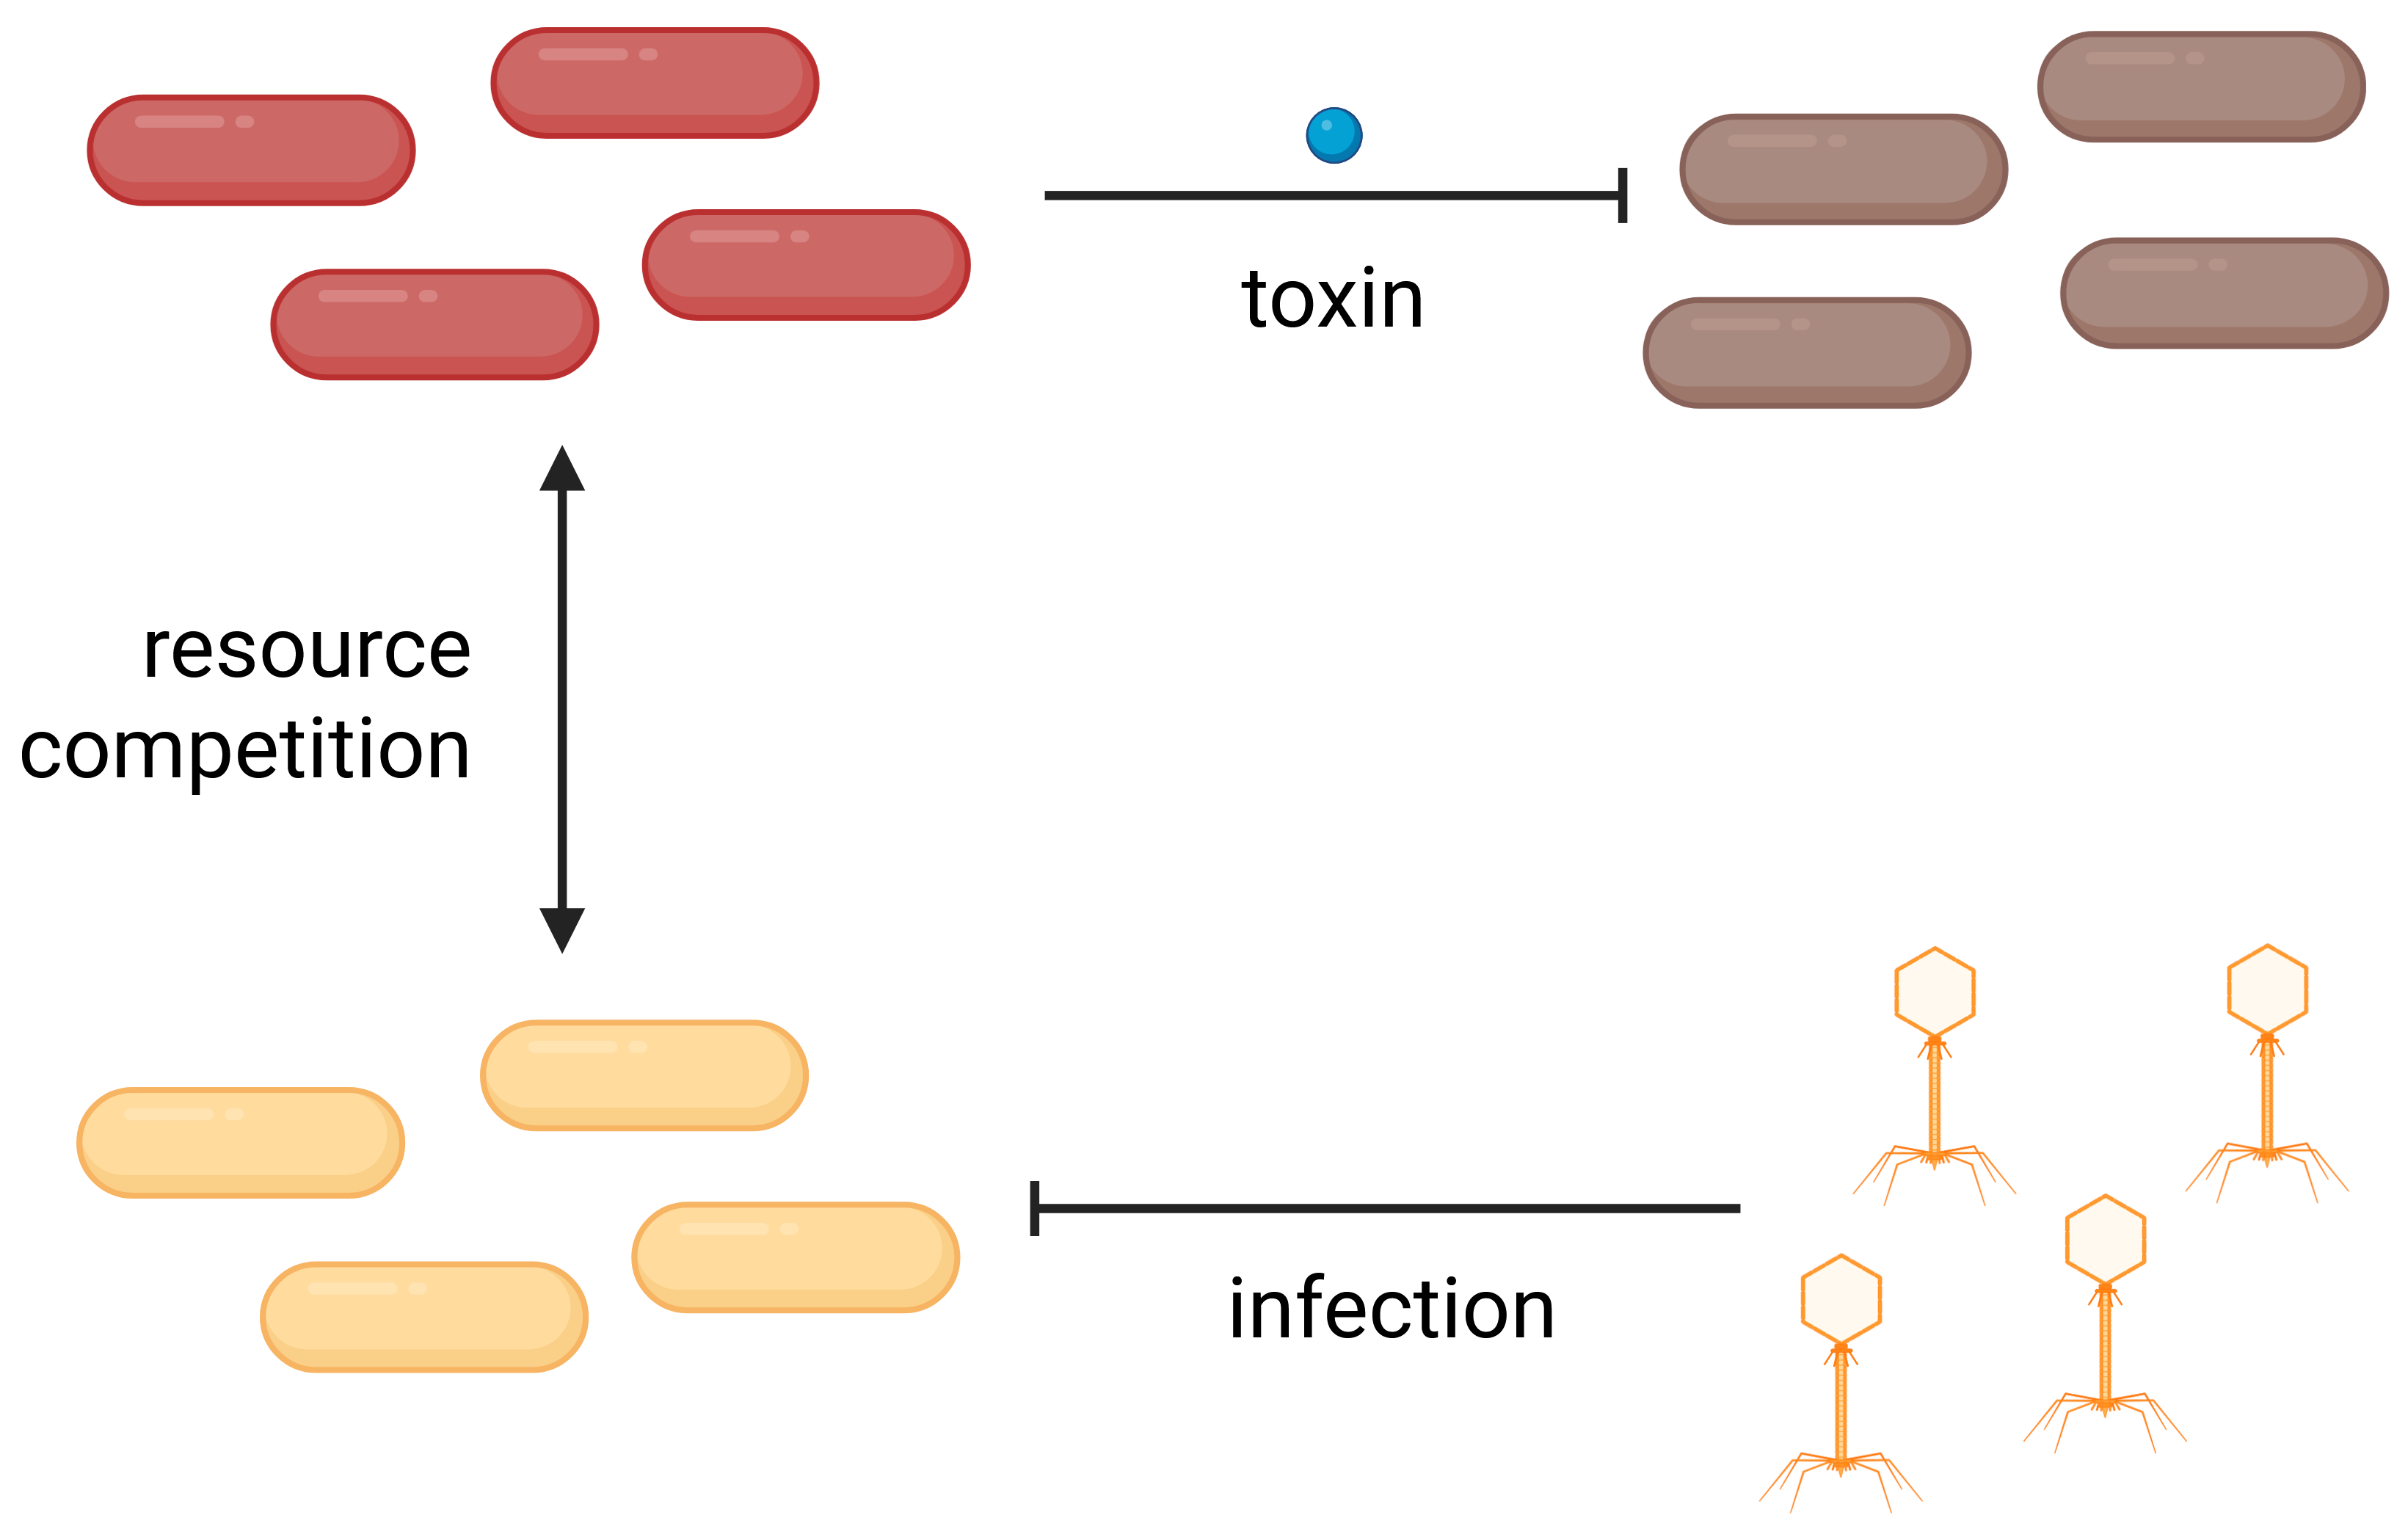
\includegraphics[width=\linewidth]{graphics/2025_09_30_intro_fig1.png}
\caption{\textbf{Antagonistic interactions studied in projects in this thesis} This sketch shows two common antagonistic interactions in microbial communities. The upper part of the sketch shows the production of a toxin by a bacterial population which can then inhibit another target strain, sensitive to the produced toxin. At the same time there are other members in the community which compete for available resources such as nutrients. This interaction will be studied in the first, experimental project of this thesis. The lower part of the sketch shows the infection of a bacterial species by phages. Phage infections form an integral, important part of natural ecology. In addition to the phage infection threat, the bacteria are in resource competition with phage-resistant bacteria. This bacteria-phage interaction will be studied in the second, theoretical project of this thesis.}
\label{fig:intro_shared_interactions}
\end{figure}

\part{Selection and evolution of antibiotic producers in microdroplets }
\chapter{Introduction}
\label{chap:droplets_intro}

This chapter introduces the relevant background and previous research for antibiotic evolution, focusing on antibiotic resistance as a global public-health concern and previous efforts to evolve antibiotic producing bacteria as well as providing reasoning, why structured environments are necessary. Furthermore, a section focuses on water-in-oil microdroplets and current technical advancements in this field. The last section describes the scope and research objectives of this project.

\section{Antibiotic resistance is a key threat in public health}

In the last decades, rapidly evolving antibiotic resistance became an increasingly important risk factor in hospital settings and later also in community environments~\cite{David2010-az}. Many efforts have been made to circumvent antibiotic resistance by optimizing treatment regimes~\cite{Kim2014-lq}, repurposing old antibiotics~\cite{Kim2019-qk} or developing entirely new drugs~\cite{Lin2017-sh} but nonetheless antibiotic resistances to clinically relevant antibiotics are commonly found~\cite{Jernigan2020-ro}. We aim to find new ways of overcoming antibiotic resistance by evolving antibiotic-producers, while specifically selecting for the increased killing of resistant bacteria.

\section{Antibiotic production in natural communities}
\label{sec:natural_production}

Natural microbial communities often include producers which gain a growth advantage over their neighboring cells by producing antimicrobial compounds. These antibiotics may give the producer a fitness advantage as they kill or inhibit the growth of its competitors in the community, often allowing the producers to use components of lysed cells as additional nutrients.
As production of an antibiotic is metabolically costly, a producer gains an advantage over neighboring cells if two criteria are fulfilled:
\begin{enumerate}
\item The concentration of the antibiotic is high enough to kill or inhibit the growth of the surrounding competitors.
\item The benefit from killing or inhibiting growth is high enough to out compete resistant, non-producing cells, which we call cheaters.
\end{enumerate}
As cheaters are not affected by the produced antibiotic but also do not produce the specific antimicrobial compounds, they may have a growth advantage over the producer and can therefore overtake the free space generated by the producer ("cheating") limiting its fitness advantage.
A long-term goal in antibiotic research is the challenge of finding conditions in which bacteria evolve to produce novel antibiotics or towards modifying existing ones, effectively emulating such natural communities.~\cite{Charusanti2012-uy} 

\section{Selection is not possible in well-mixed environments}

The effect of an antimicrobial compound in spatially structured environments is limited by diffusion to the immediate surrounding of the producers. Therefore one only sees a growth inhibition zone in close proximity to a colony of producers. One could think that using a well mixed environment could increase the effect of the antibiotic.
However, due to the constant mixing in a well-mixed environment, the produced antibiotic is usually dispersed through the entire culture and does not accumulate to a high enough concentration required to actually kill competitors as sketched (not to scale) in figure~\ref{fig:intro_droplets_idea}a. Moreover, even if the antibiotic accumulates to a high enough concentration (due to high production rates or a large number of producing cells) the chance of an existing cheater growing equally fast or even faster than the producer is close to 1.
Therefore, according to the criteria defined in section~\ref{sec:natural_production}, producers do not have a growth advantage over other cells in well mixed environments and are usually not selected for or even out-competed by cheaters due to the significantly lower growth rate as a result of the antibiotic production.

\section{Spatial structures enable selection for antibiotic producers}
\label{sec:spatial_structure}

Agar plates as spatially structured environments were successfully used in a previous study to show that producers have a growth advantage compared to cheaters when grown in competition with sensitive cells (the colonies of producers are bigger than the ones of cheaters). However, as soon as a cheater is in close proximity to a producer (within the inhibition zone of the latter one), it will profit from the killing of the sensitive cells. Therefore one can only work with very low densities of producers on agar plates to minimize the probability of a cheater to be in the inhibition zone created by a producer~\cite{Gerardin2016-ac}. The small population size available in this setting limits the potential for de novo mutations which would lead to evolution of the antibiotic producer.

\begin{figure}
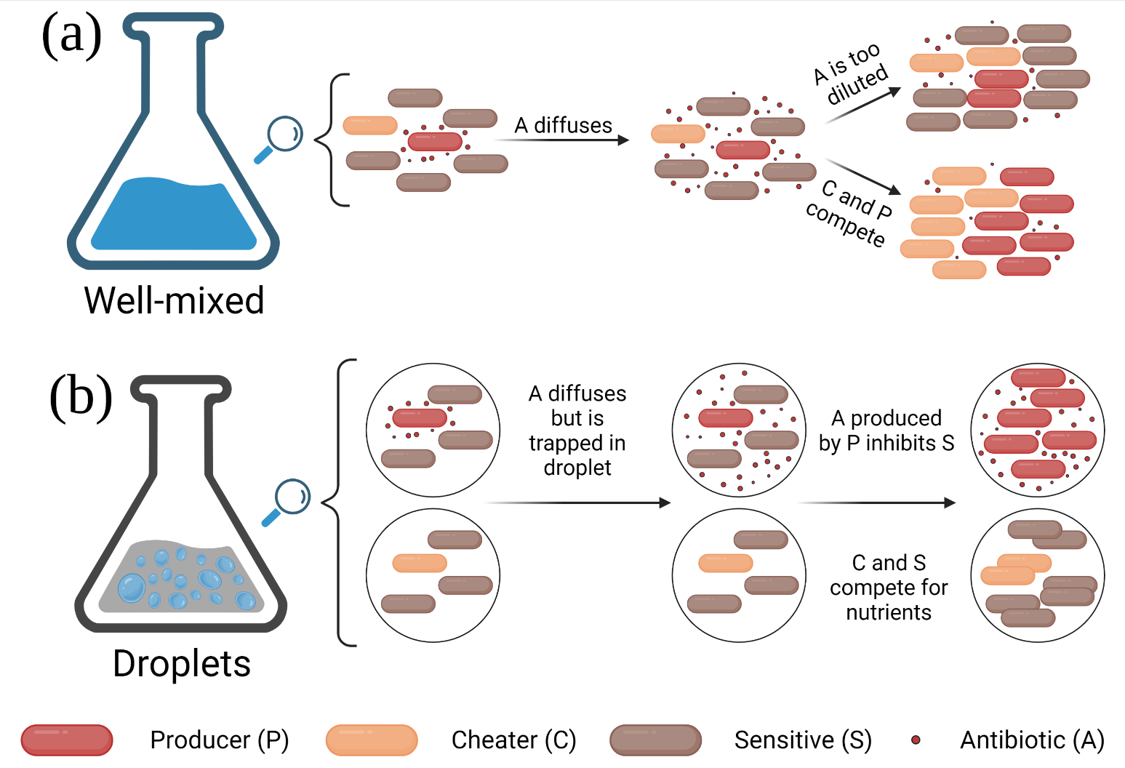
\includegraphics[width=\linewidth]{graphics/2025_09_28_droplets_fig1_new.png}

\caption{\textbf{Microdroplets provide a platform for selection of antibiotic producing cells.} In this sketch, the interactions between sensitive (blue), producing (dark red) and cheating (light red) cells in a well-mixed (a) and in a water-in-oil droplet (b) environment are shown. \textbf{(a)} Upon production of the antibiotic (red crosses), it is immediately dispersed through the entire culture due to constant mixing. Two possible outcomes are possible, as sketched here. In the first outcome, the antibiotic is too diluted to inhibit growth (as shown in the upper part) and all cells grow at a similar rate. In the second outcome, the antibiotic is highly concentrated and kills the sensitive cells in the entire culture as shown in the lower part. Due to the killing of all sensitive cells, the cheater cells can equally profit from the absence of the sensitive cells and both, producers and cheaters, grow. \textbf{(b)} In droplets producers and cheaters can be separated in different droplets as depicted here. The producer will target sensitive cells trapped in the same droplet as the antibiotic molecules cannot disperse through the entire culture (into other droplets). So the producer is the only cell which profits from the effect of the antibiotic and grows faster than cheaters and sensitive cells in competition in other droplets as depicted in the last step.}
\label{fig:intro_droplets_idea}
\end{figure}

\section{Water-in-oil microdroplets as a technology for \\ high-throughput spatially structured microenvironments}

In recent years, microdroplets have become a commonly used technology in biomedical applications~\cite{Zagnoni2011-ko}. They enable us to encapsulate small volumes $ \left( \approx 50 \mathrm{pl} \right)$ of growth medium and competing cells in separate microenvironments as sketched in figure \ref{fig:intro_droplets_idea}b. Due to the high generating frequency in microfluidic chips, currently accessible $\left( \approx 10^4 \frac{\mathrm{droplets}}{\mathrm{s}} \right) $, we can now perform high-throughput experiments.
Therefore, with microdroplets, we can replace the problem mentioned in section~\ref{sec:spatial_structure} of a limiting density of producers on agar plates with the problem of a limiting concentration of producers in the aqueous phase which can more easily be dealt with by producing more droplets, which is a matter of time rather than a matter of space as it was on agar plates~\cite{Gerardin2016-ac}. Having longer production times for droplets would increase the number of produced droplets by up to $10^4$ droplets per second.
Assuming the chance for a mutation which modifies antibiotic production to be $10^{-8}$~\cite{Drake1998-es, Kunkel2004-br, Wielgoss2011-jd} and our ability to easily reach $10^7$ droplets in a reasonable time, we can considerably increase the chance of obtaining such mutations compared to agar plates used previously, where the maximal number of distinct colonies reached $10^3$~\cite{Gerardin2016-ac}.

\section{Scope and objectives of the project}

The project has three main objectives:
(1) We will establish a high-throughput microdroplet system to select for antibiotic producing cells.
(2) We will select for the antibiotic producing cells in competition with sensitive and cheater cells in microdroplets.
(3) We will find evolutionary pathways leading to de novo mutations within the antibiotic producing cells which help overcoming evolved resistance.
By evolving the antibiotic to target resistant cells, we would be able to isolate the antibiotic from its producer in a next step as done before~\cite{Singh2018-qp} and one could conduct clinical studies to use this antibiotic in patients treatment. The project would serve as a proof-of-principle how one could try to target the increasing threat of antibiotic resistances.
The resulting mutations could offer a general way to improve antibiotics effectiveness which is not known yet and therefore could lead to new opportunities of generating new, enhanced antibiotics which can be used to treat infections with resistant bacterial strains.
We expect this project to have a significant impact on how we currently think about evolvability of antibiotic producing cells and how these obtain de novo mutations which give a fitness advantage. Furthermore, we expect to gain insight into the dynamics of an arms race between antibiotic producing and resistant cells and therefore understand the key principles of how resistance evolves in the presence of antibiotic producing cells.


\chapter{Methods}

\section{Bulk droplets}

\section{On-chip droplets}
Using a commercially available microfluidic chip (Dolomite)
\section{Halo assay}

\section{Liquid and droplet comparison}

\section{Conditional medium}
\chapter{Results}

This chapter will present the partial results we obtained in this project. First, we will present the different technologies we used in producing droplets and how we overcame arising technical challenges. Then we introduce how we identified an antibiotic producer and its respective target using halo assays to conduct a library screening. Lastly we focus on biological problems which arose due to the unique nature of the droplet environment and issues with the chosen antibiotic production strain in general which led us to conclude the project. 

\section{Successful droplet production}
\begin{figure}
\centering
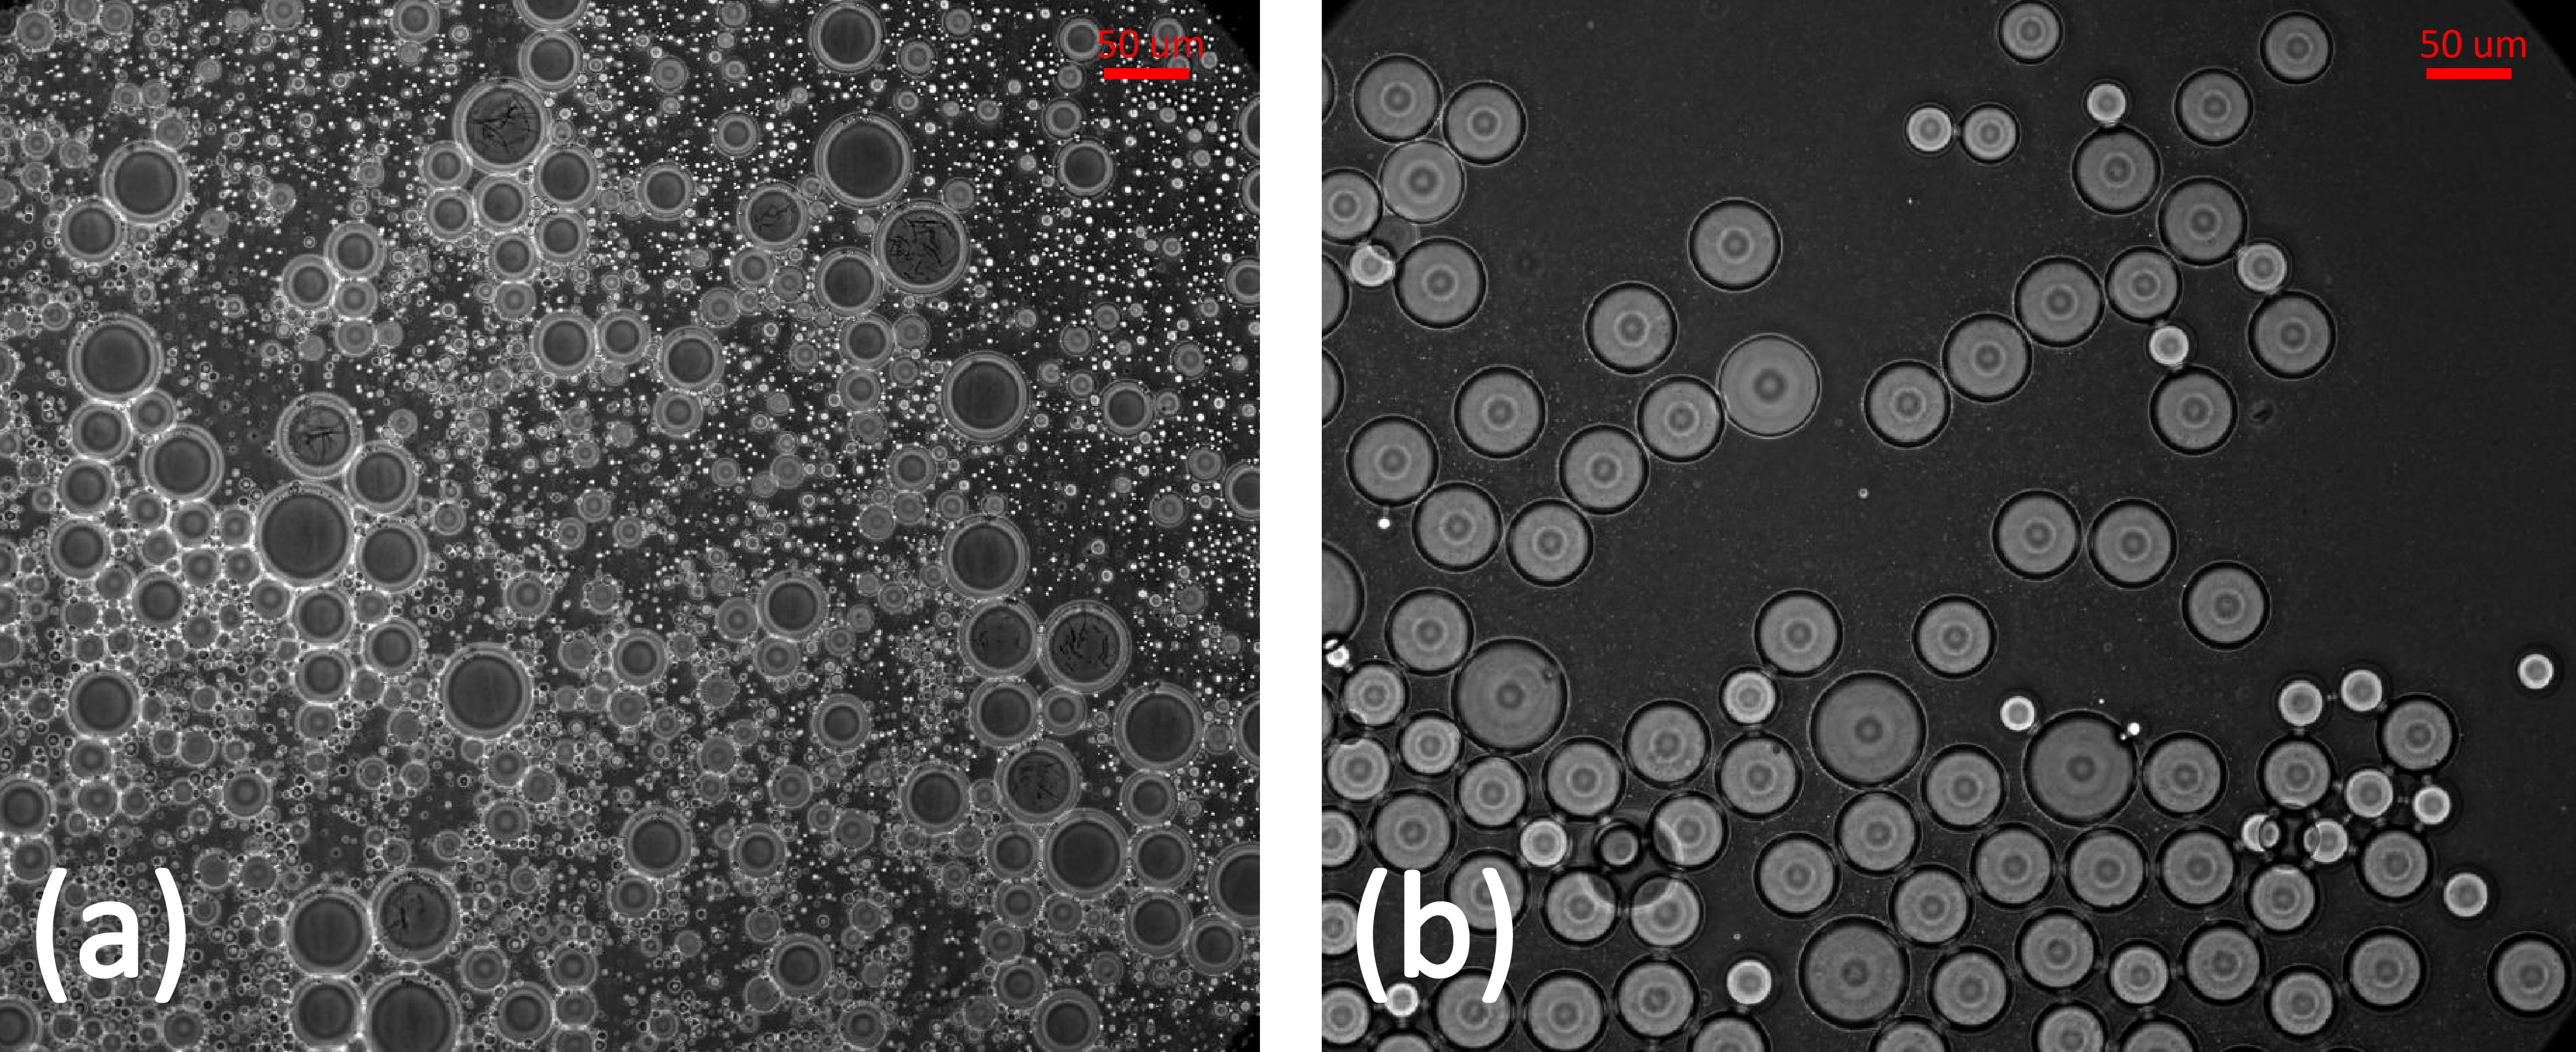
\includegraphics[width=\linewidth]{graphics/2025_09_30_droplets_fig5.png}
\caption{\textbf{Comparison of bulk droplets and on-chip droplets reveals broad size distribution in bulk droplets and narrow size distribution in on-chip droplets} In (a) we see bulk microdroplets after 21h of incubation (30$^\circ$C). A broad distribution of droplet sizes can be observed. In bigger droplets, bacteria are observed. In (b), we see on-chip microdroplets. These are more uniform in size, especially a lower size limit can be observed and the bigger droplets are probably merged single droplets.}
\label{fig:results_droplet_bulk_vs_chip}
\end{figure}
We employed both methods, described in sections~\ref{sec:method_bulk_droplets}~and~\ref{sec:method_chip_droplets}, to produce droplets successfully.~Figure~\ref{fig:results_droplet_bulk_vs_chip} shows the resulting droplets from employing both methods. When using magnetic stirrers to create bulk droplets, we obtain stable microdroplets which are stable even over longer periods of time and incubation. The size distribution is very broad and the upper limit allows significant bacterial growth in droplets~(Figure~\ref{fig:results_droplet_bulk_vs_chip}a). In contrast to this method, when using a commercially available microfluidic chip, we can produce droplets with a very narrow size distribution~(Figure~\ref{fig:results_droplet_bulk_vs_chip}b). These droplets also allow for bacterial growth but producing the droplets is more challenging due to sensitivity of pressures and possible accumulation of debris in the chip which can block production. Nevertheless, for our pilot experiments we use the microfluidic chip to improve reproducibility of droplets and experiments.

\section{Recommended oil evaporates rapidly}
\begin{figure}
\centering
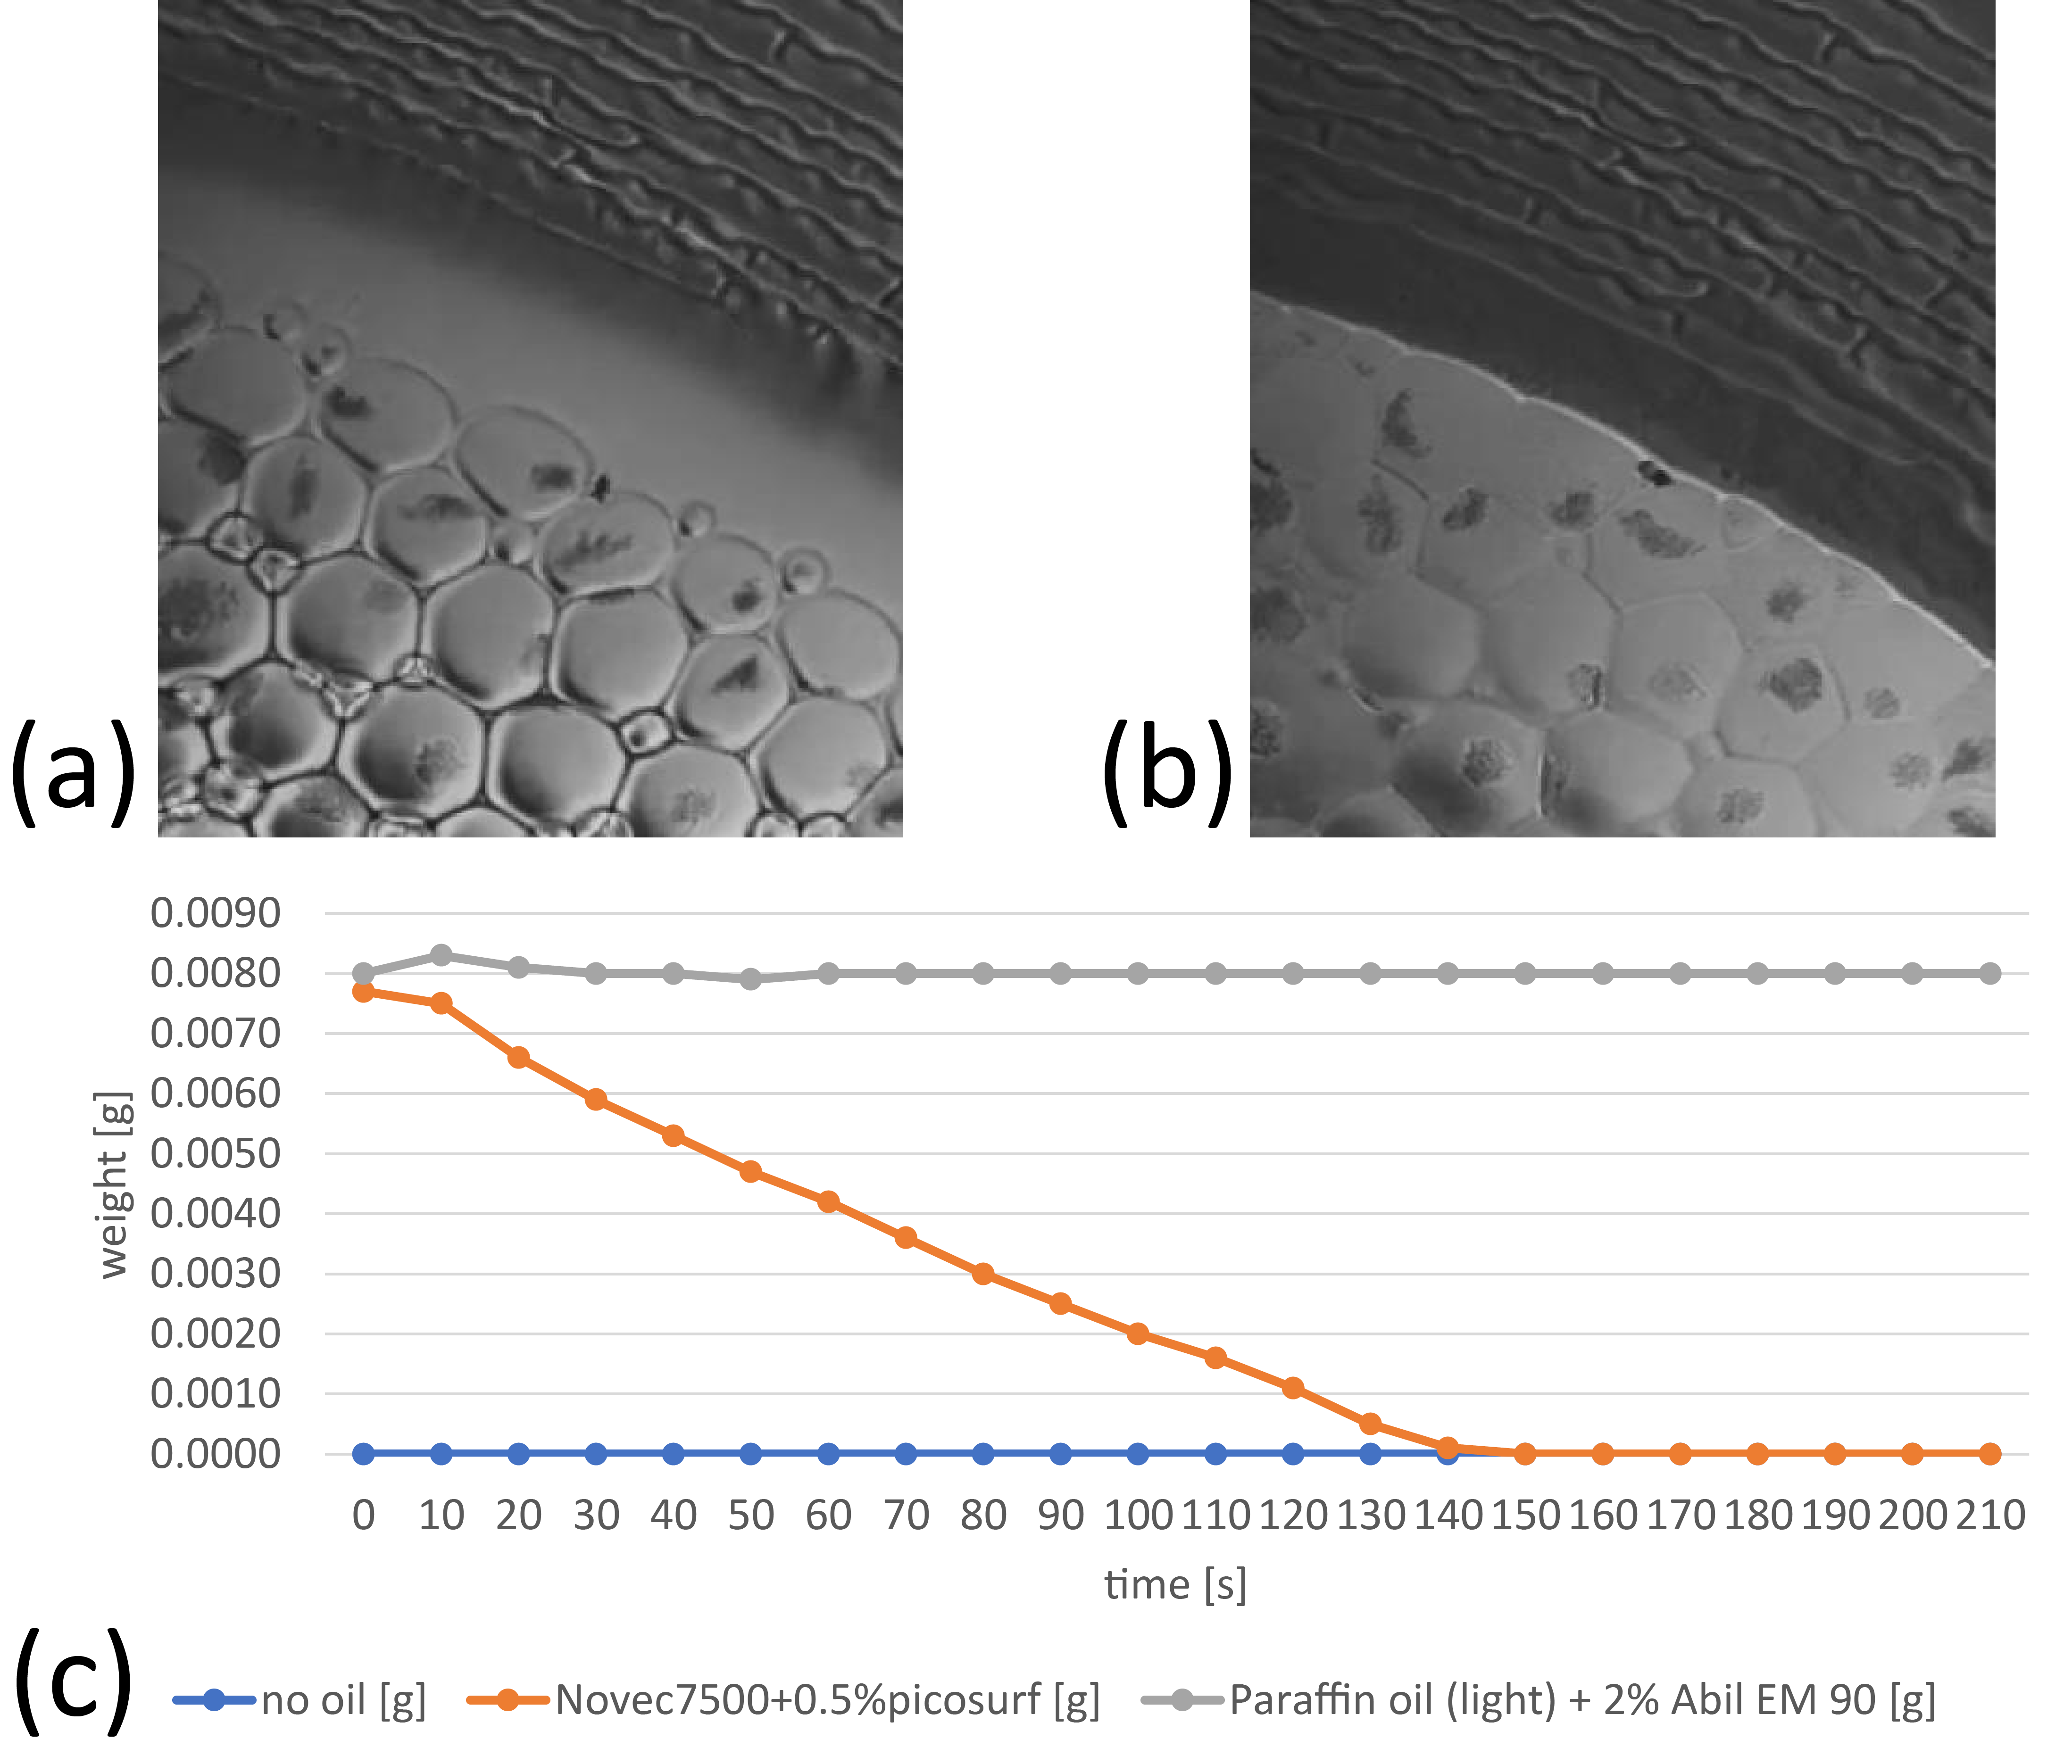
\includegraphics[width=\linewidth]{graphics/2025_09_30_droplets_fig6.png}
\caption{\textbf{Novec\textsuperscript{TM}7500 rapidly evaporates and does not allow for droplet incubation and observation} Using a recommended oil for the commercial microfluidic chip we used, we observed oil evaporation. (a) and (b) show two snapshots of droplets after 21h of incubation in a sealed flask upon placing under the miroscope. The oil recedes (a) until it completely evaporates and the droplets merged (b). Measuring the oil weight on a scale shows a decrease of oil over time (c) while Paraffin oil does not evaporate on the same time scale.}
\label{fig:results_oil_evaporation}
\end{figure}
While we were able to produce stable, observable droplets using Paraffin oil, we did not succeed to observe droplets using Novec\textsuperscript{TM}7500 which was recommended by the manufacturer of our microfluidic chip. Interestingly, we were able to produce droplets and incubate them over long time. Yet, upon exposure to air, the oil exhibited wave dynamics when observed under a microscope (Figure~\ref{fig:results_oil_evaporation}a) and after a short time, the droplets got pushed together and finally surface tension led to collapse and merging of the distinct droplet environments (Figure~\ref{fig:results_oil_evaporation}b). This led us to suspect that the oil might evaporate in our conditions and indeed, when using a glass slide on a high-precision scale and adding a $5 \mu l$ drop of oil, we observe a rapid weight loss, indicating evaporation. For Paraffin oil, which we also use to create droplets, we do not observe this phenomenon~(Figure~\ref{fig:results_oil_evaporation}c). Thus, we focused on producing droplets solely with Paraffin oil.

\section{Identifying producer-target pair}
\begin{figure}
\centering
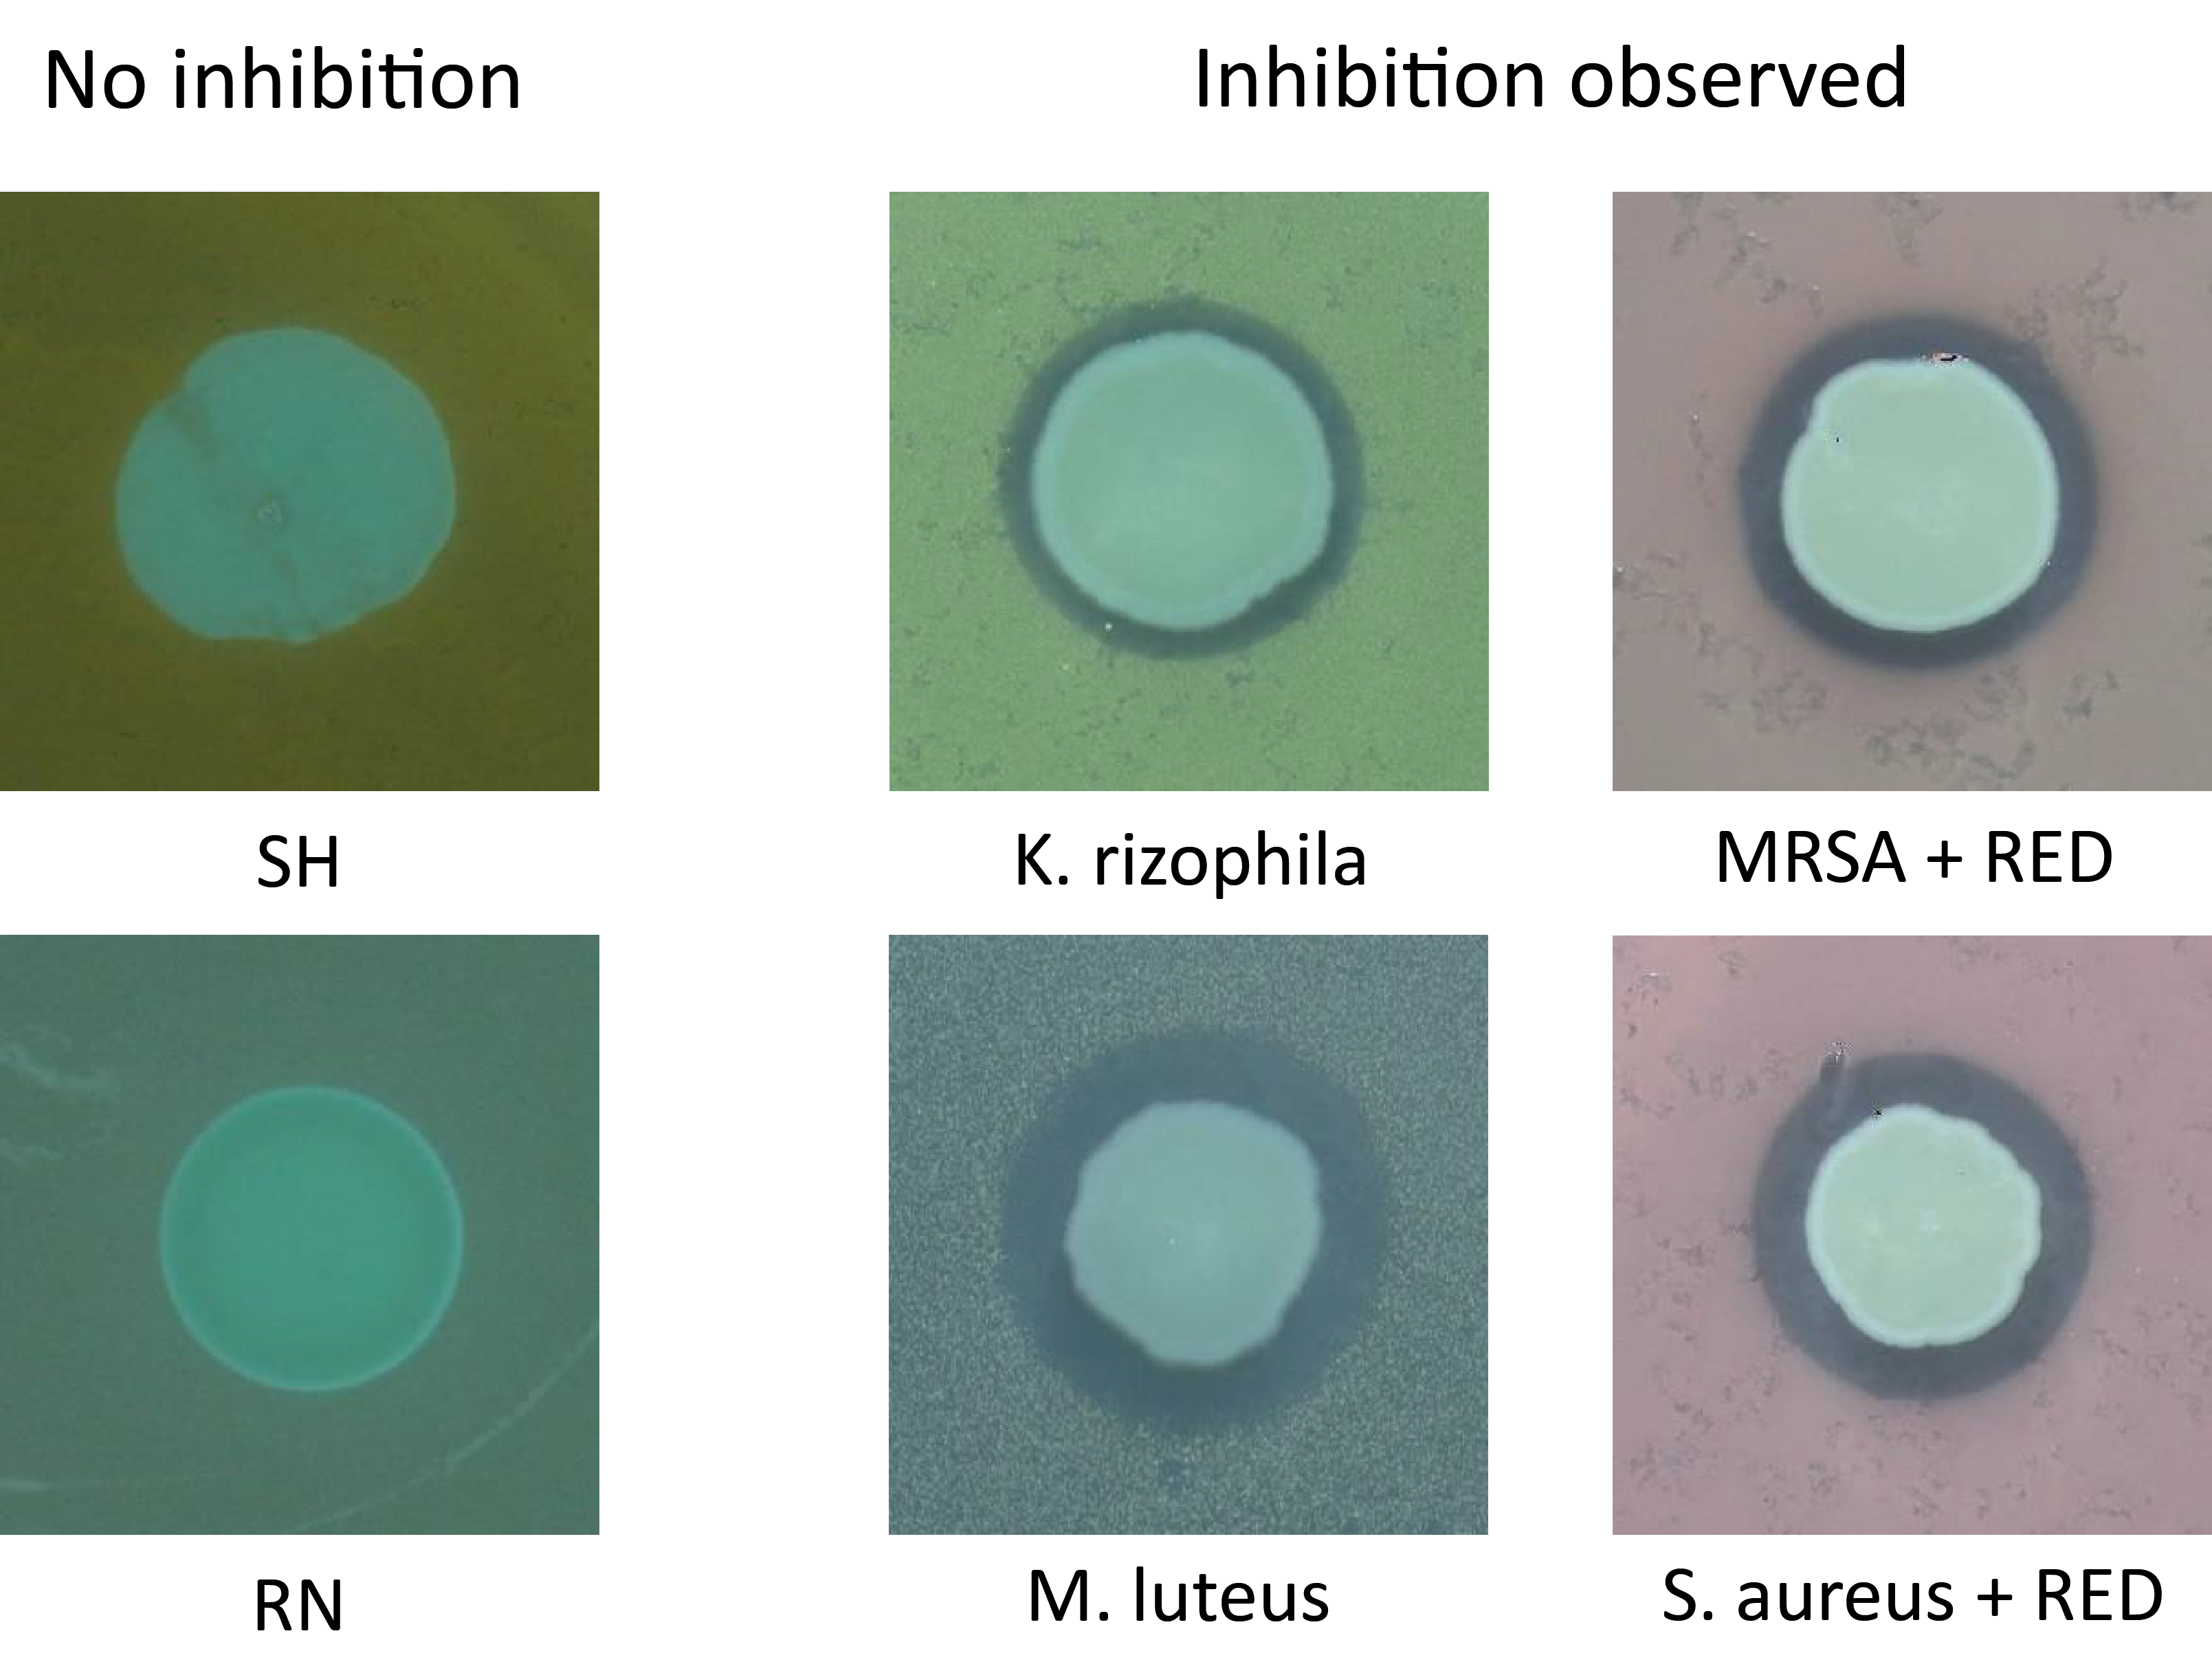
\includegraphics[width=\linewidth]{graphics/2025_09_30_droplets_fig7.png}
\caption{\textbf{Halo assay for library of target strains identifies \textit{Staphylococcus aureus} as potential target} Using halo assays, we conducted a broad screening of very distinct bacterial strains to determine possible target strains for the chosen \textit{Bacillus subtilis} producer strain. Some natural isolates from our collection showed no inhibition but we observed several strains which exhibit inhibition. Among them the commonly used susceptibility test strain of \textit{Kocuria rhizophila} but also clinically relevant strains of \textit{S. aureus}, both methicillin-resistant (MRSA) and sensitive.}
\label{fig:results_sensitive_screening}
\end{figure}
Previous research in our lab~\cite{Gerardin2016-ac} used a colicin-producing \textit{E. coli} strain as an antibiotic producing strain. This is less feasible in droplets due to the inherent nature of colicin. In order for bacteria to release colicin, these bacteria need to lyse~\cite{Cascales2007-oj}. As the volume in droplets is very limited, we inoculate the droplets with low numbers of bacteria. The need of lysis does not allow to use colicin in our setup.
Instead we focused on other antibiotics, based on several criteria like culturability in growth media also suitable for possible target strains, small molecule antibiotics, to allow for beneficial mutations and some hydrophilicity to avoid diffusion outside of the droplets. Based on these criteria, we chose a subtilin-producing \textit{B. subtilis} strain~\cite{Stein2002-nv, Zhang2022-ee} as the antibiotic producing strain.
After choosing our antibiotic producing strain, we screened a collection of possible target strains, selected based on similar growth rate and easy culture conditions using halo assays. We observe inhibition for several of the possible targets~(Figure~\ref{fig:results_sensitive_screening}). Based on these results, we chose a \textit{Staphylococcus aureus} strain due to the large inhibition zone combined with its clinical significance.

\section{\textit{Bacillus subtilis} stressed in droplets}
\begin{figure}
\centering
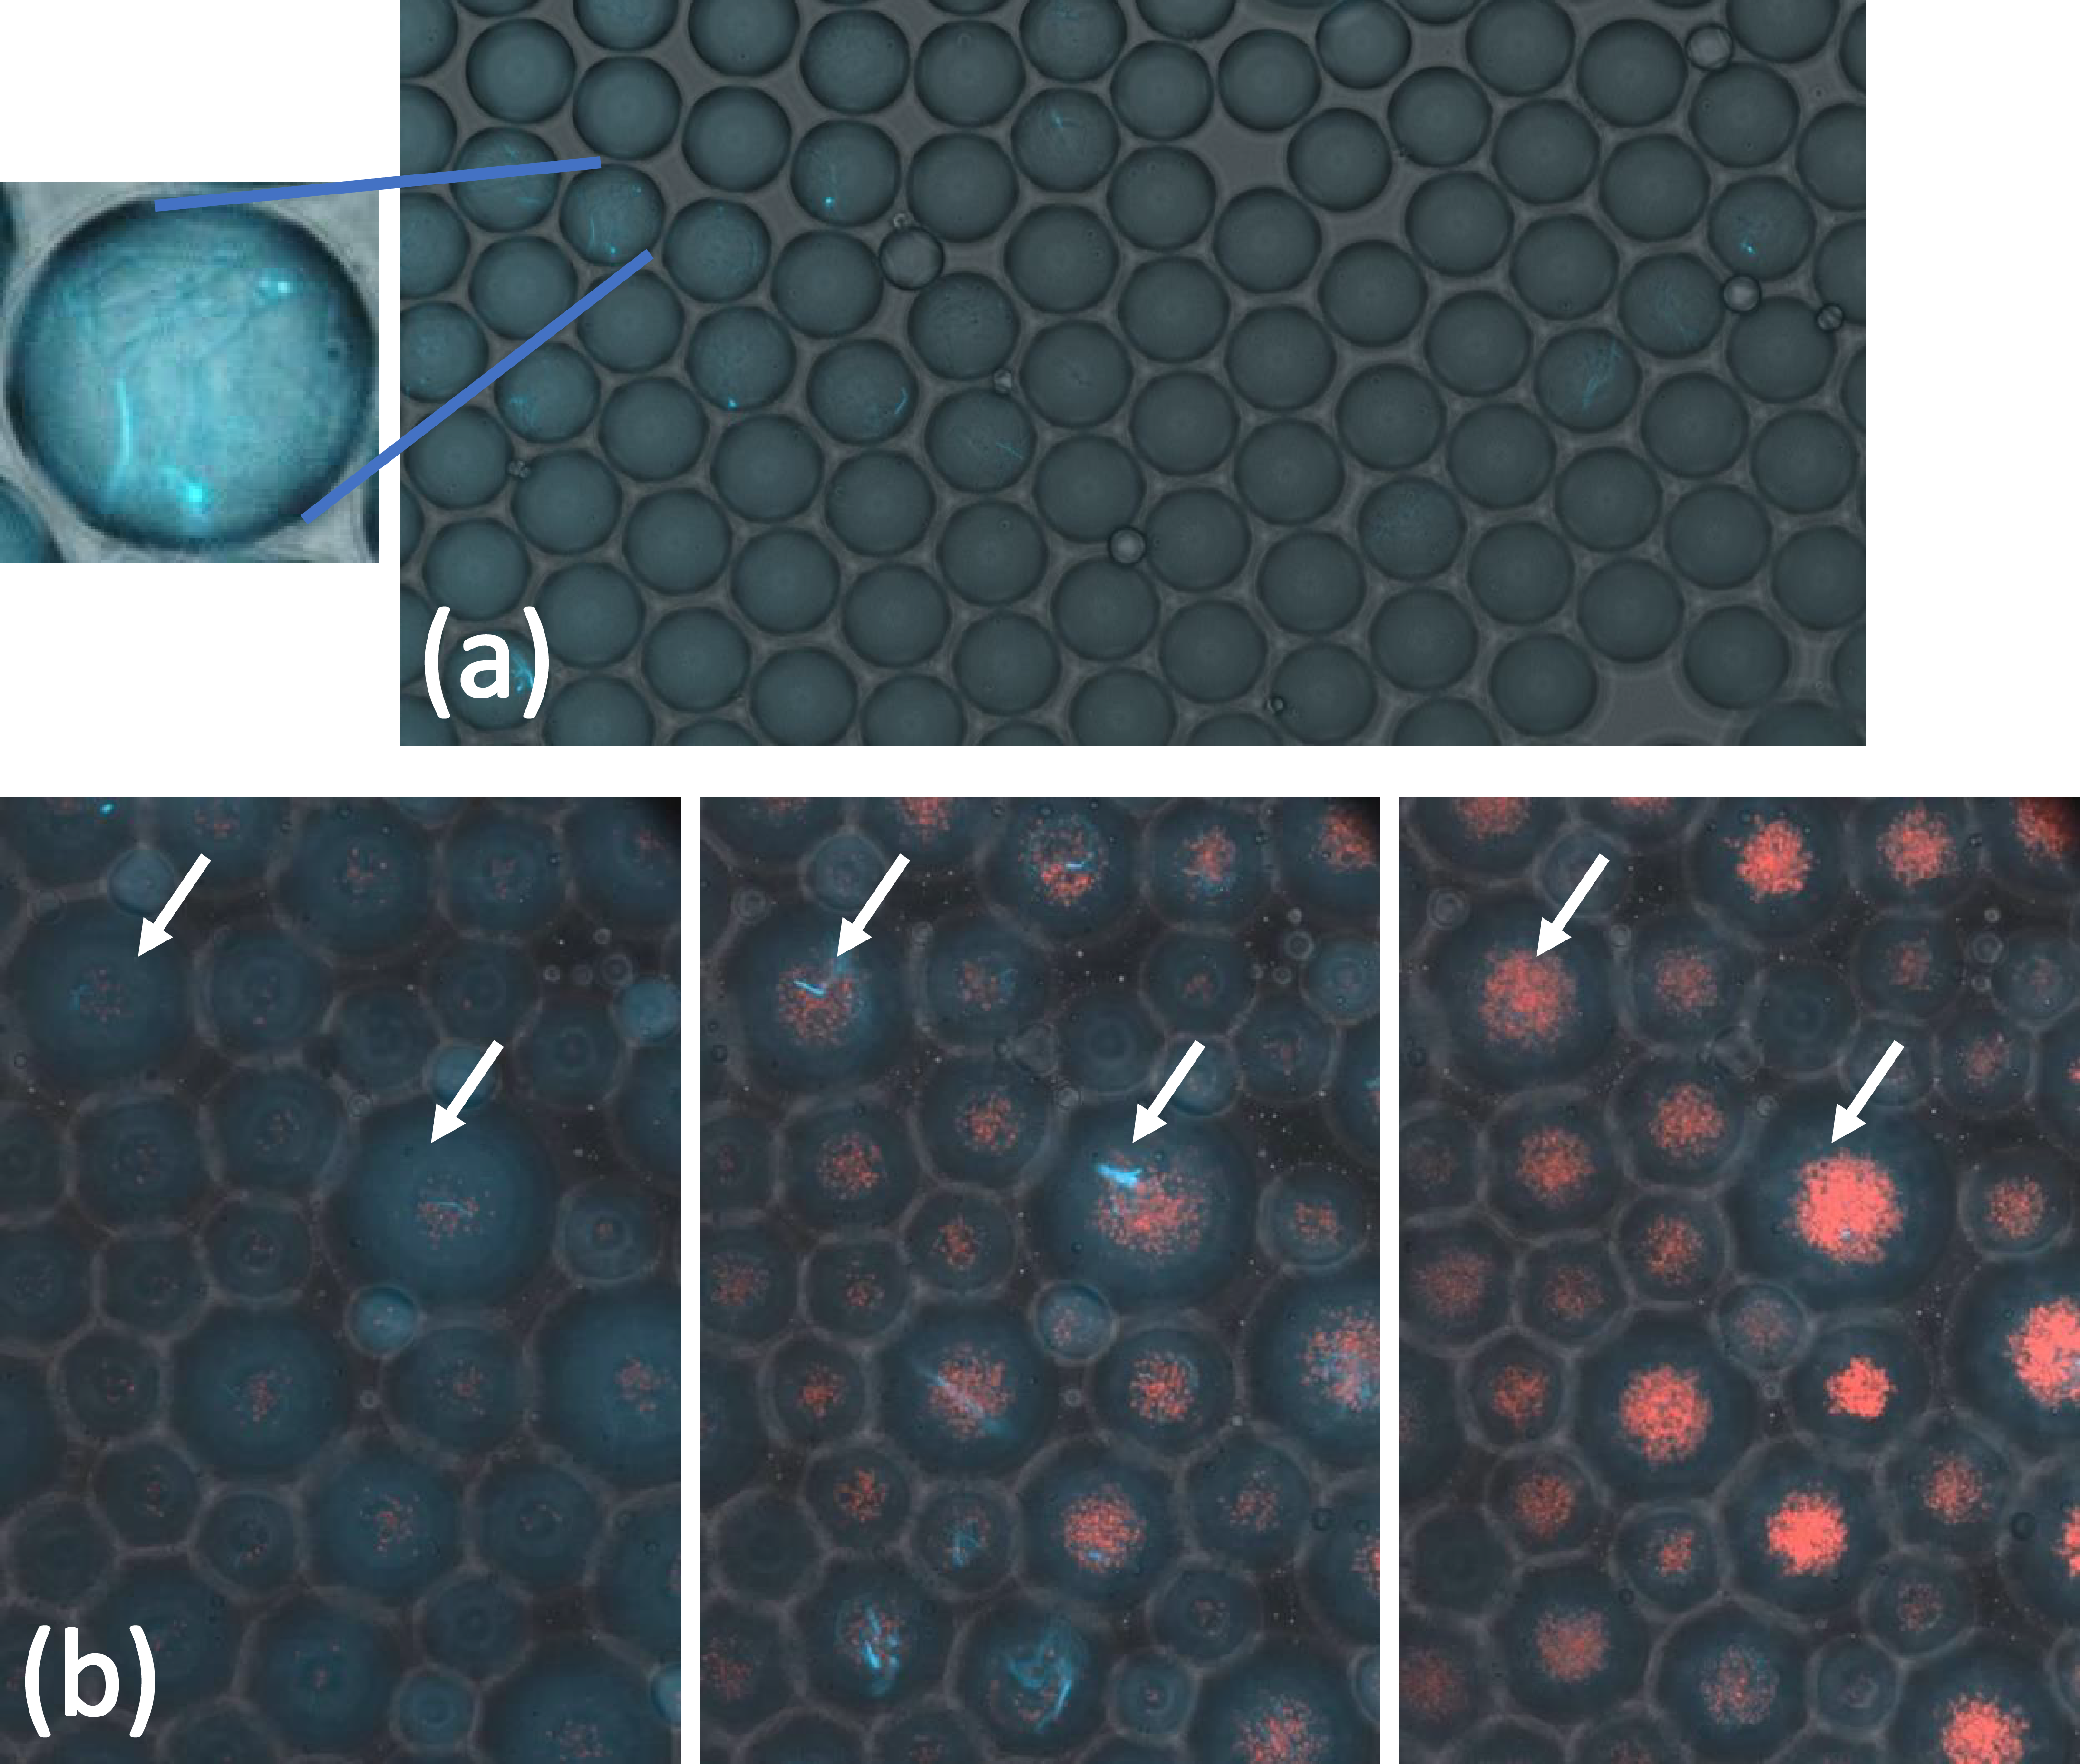
\includegraphics[width=\linewidth]{graphics/2025_09_30_droplets_fig8.png}
\caption{\textbf{On-chip droplets are stable after long-term incubation and allow bacterial growth} Our setup allows for long-term incubation and monitoring of droplets. (a) shows the results after 21h of incubation of droplets containing antibiotic producers alone in 30$^\circ$C. We observe stable same-sized droplets containing fluorescently tagged bacteria. The bacteria seem to be stressed and filament in the droplets as can be seen in the contrast and brightness enhanced enlarged droplet on the left. (b) shows snapshots of a time series of droplets containing both, antibiotic producing \textit{B. subtilis} (tagged in blue) and sensitive \textit{S. aureus} (tagged in red). Initially we see growth of both bacterial strains. However, \textit{B. subtilis} seems to be filamenting (examples indicated with arrows) and at the end of the incubation, most droplets are filled exclusively with the target \textit{S. aureus} strain.}
\label{fig:results_incubation_subtilis}
\end{figure}
After establishing the technical platform, we can incubate droplets for long periods of time and can monitor them under the microscope during these incubation periods~(Figure~\ref{fig:results_incubation_subtilis}). We encapsulate the antibiotic producer alone~(shown after incubation in Figure~\ref{fig:results_incubation_subtilis}a) and together with the target strain (time series in Figure~\ref{fig:results_incubation_subtilis}b) in droplets. Encapsulating it alone, we observe long filaments of cells in the droplets after incubation as the enlarged, contrast and brightness enhanced droplet in the figure shows. This indicates some kind of stress in this specific growth environment. When encapsulating it together with sensitive bacteria, we observe droplets with antibiotic producers and target cells and some only with target cells, in line with the chosen concentrations. After initial growth, we observe filamenting antibiotic producers (marked with white arrows in the time series in Figure~\ref{fig:results_incubation_subtilis}b) and after 21h of incubation, the antibiotic producers disappeared almost completely from the droplets (Figure~\ref{fig:results_incubation_subtilis}b, right side), while the target cells grow properly in the droplets. Together with the observation of filaments in droplets where antibiotic producers are encapsulated alone, this might indicate the lack of toxin production and the lack of growth of antibiotic producers in droplets.

\section{Comparison of growth in liquid and droplet environment}
To understand if the antibiotic producer disappears only in droplets or also in liquid, we performed a liquid-droplet comparison assay with separate cultures of antibiotic producer and the target strain. After incubation for 21h with high inoculation densities, we see that both liquid cultures exhibited growth while in droplets only the target strain exhibits growth. The antibiotic producer seems to not grow in droplets during the incubation period but rather seems to reduce in population size~(Figure~\ref{fig:results_liquid_vs_drop_supernatant}a).

\begin{figure}
\centering
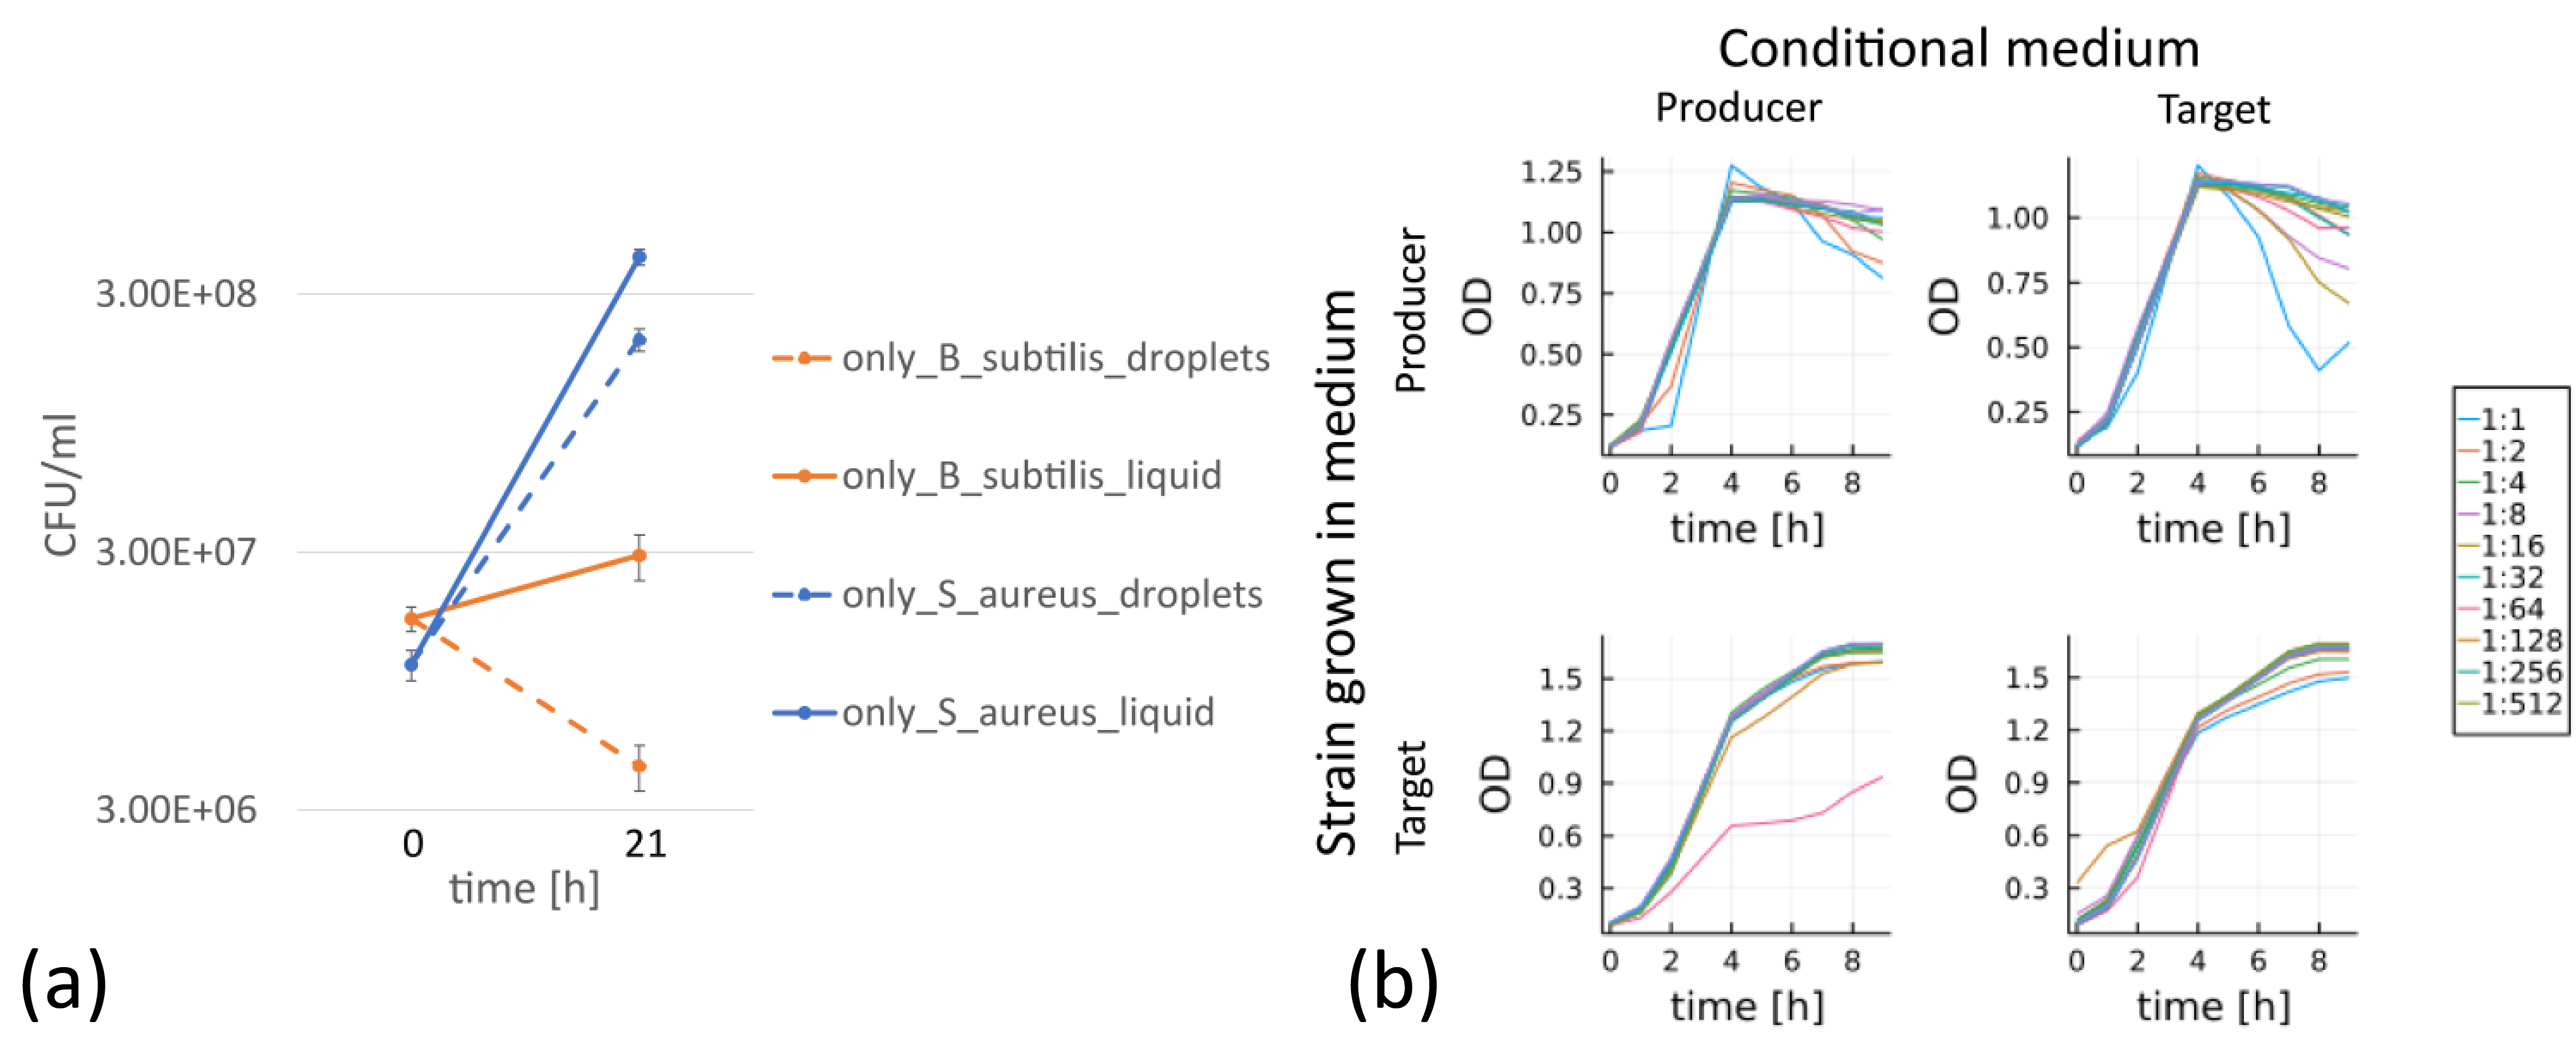
\includegraphics[width=\linewidth]{graphics/2025_09_30_droplets_fig9.png}
\caption{\textbf{\textit{B. subtilis} fails to grow in droplets and does not kill in liquid} To understand the observed dynamics in droplets, we conducted liquid experiments. (a) shows the results of comparing growth of antibiotic producing \textit{B. subtilis} alone (orange) in liquid (solid line) and in droplets (dashed line) and similarly for the target \textit{S. aureus} strain (blue). We observe that \textit{B. subtilis} seems to die in droplets while it grows in liquid culture. \textit{S. aureus} seems to grow almost equally well in droplets and liquid culture. (b) shows the results of growing bacteria in conditional medium. Studying both, antibiotic producer and target strain conditional media, we do not observe an effect of the antibiotic in liquid, hinting at the possible absence of antibiotic in liquid compared to growth on agar.}
\label{fig:results_liquid_vs_drop_supernatant}
\end{figure}

\section{Chosen antibiotic producer does not produce sufficient antibiotic to kill target strain in conditional medium}
To measure the effectivity of the produced antibiotic, we use a conditional medium assay. We grow producer and target on its own or the other strain's conditional medium respectively. We do not observe a significant impact of the conditional medium on growth of bacteria in any of the conditions~(Figure~\ref{fig:results_liquid_vs_drop_supernatant}b), especially when growing the target strain on the conditional medium of the antibiotic producing strain~(Figure~\ref{fig:results_liquid_vs_drop_supernatant}b, bottom left). This indicates the lack of significant antibiotic production by the producer when grown in liquid, rendering it unusable in a droplet encapsulation scenario.
\include{main_droplets/mainchap1}
\chapter{Conclusion and open questions}
\label{chap:droplets_conclusion}

We were able to produce stable droplets in which we were able to incubate bacteria overnight...

However, after selecting a pair of bacterial strains which exhibit a antagonistic interaction on solid growth medium, we were not able to grow the antibiotic producing strain of \textit{B. subtilis} successfully in droplets and furthermore, we failed to induce antibiotic production and accumulation in liquid.
Further research should investigate other pairs of strains exhibiting antagonistic interactions and first verify that inhibition also happens in liquid culture and both strains grow successfully in droplets before moving to produce droplets with competing bacteria.

%
% and then cover:
% - The methods used in the research
% - The research results
% - Discussion and conclusions from the results
%
% but not necessarily with a specific chapter for each of them.
%
% Then you have your main chapters (although these might still
% include an initial chapter on technical preliminaries, experimental
% system setup, and/or a final chapter with summary, discussion and further
% research direction or questions)

\part{Simulating bacteria-phage interactions}
\chapter{Introduction}
\label{chap:intro}
% % do we need to add TOC lines?

% %\begin{figure}
% %  \centering
% %  \includegraphics[width=0.75\textwidth]{main/graphics/a_blowup.pdf}
% %  \caption{This is a caption}
% %\end{figure}

% Here you can introduce the field, survey past results, give context, use citations of course... (e.g. \cite{CLR}). It is probably worthwhile to clarify the goals or targets of the research and describe the process, unless this is done later.

% You can also introduce \emph{a key concept} (or rather, several) without formally defining them until later on.

% \subsection*{An unnumbered subsection}

% You may want to break up the intro into parts with titles. Subsectioning without numbering is an option you might want to consider.

% Some people include a specific section overviewing the results ("In Chapter so-and-so, we will see how etc.") which is also a way of describing the structure of the thesis. But this is not necessary.

% \subsection*{Thesis options and appearance}

% Please note that the \texttt{iitthesis} class has several options when you use it, such as:
% \begin{itemize}
% \item \texttt{fullpageDraft} to avoid the margins necessary for proper binding when you make the final print
% \item \texttt{beforeDefense} makes the personal acknowledgements invisible; use this to print the copies you submit initially to the grad school for sending to the opponent panel, i.e. thesis readers (who shouldn't see those parts). For the final submission, after having successfully defended --- drop this option. 
% \item \texttt{noabbrevs} no notation \& abbreviations list will be included in the thesis.
% \end{itemize}

% \subsection*{Hebrew font}

% The \texttt{iitthesis} document class uses the David CLM font family for Hebrew text. CLM is a shorthand for ``Culmus'' (\texthebrew{קולמוס}) --- the name of a freely-available Hebrew font package. It may be bundled with your LaTeX distribution, or otherwise, must be available as system fonts. If you're missing the Culmus fonts, try adding an appropriate package from your LaTeX distribution or system distribution; alternatively, you might want to visit the Culmus project page at \url{http://culmus.sourceforge.net/} and download and install the fonts manually.

% \subsection*{Setting thesis meta-data and publication information}

% The document class used to generate this document defines several commands you can use to set information  regarding your thesis, which is used in the title pages and elsewhere in the front matter.  Every (or almost every) command has an English and a Hebrew variant, with a \texttt{English} or \texttt{Hebrew} suffix to the command name. Examples:
% \begin{itemize}
% \item \verb|\titleHebrew|, \verb|\titleEnglish|
% \item \verb|\authorHebrew|, \verb|\authorEnglish|
% \item \verb|\JewishDateHebrew|, \verb|\JewishDateEnglish|
% \item \verb|\GregorianDateHebrew|, \verb|\GregorianDateEnglish|
% \item \verb|\publicationinfoHebrew|, \verb|\publicationinfoEnglish|
% \end{itemize}

% The file \texttt{misc/thesis-fields.tex} contains invocations of several such commands (some of them commented-out with \texttt{\%}), and some additional information about them.

This chapter introduces the key biological concepts for this project, namely bacteriophages and their interaction with bacteria. Furthermore, this chapter introduces the importance of spatial structure in natural environments and its impact on ecological dynamics. Lastly, we introduce reaction-diffusion equations, the class of computational models used in this project to simulate dynamics in a spatially structured environment and we highlight some applications of such models.

% \section{General overview}

% Over the last decades, bacteria and bacteriophages (phages) became a model system to study host-parasite interactions, however they were lagging behind other systems in understanding their coevolution and ecology~\cite{Koskella2014-yp}.
% Despite the early proof that bacteria and phages can coexist in liquid media~\cite{Chao1977-rj}, it was also early on shown that evolution stagnates rapidly in these chemostat cultures~\cite{Lenski1985-wb} and different explanations were proposed why a continuous coevolution is not taking place~\cite{Lenski1984-ei}, recent experiments and models started taking spatial structure of the system's environment into account given the prevalence of spatial structure in natural environments such as biofilms~\cite{Krysiak-Baltyn2016-xi, Gourley2004-rx}. Most work in spatially structured systems focuses on ecological interactions and does not involve possible evolution which might influence the dynamics through evolution. Recent experimental work~\cite{Shaer-Tamar2022-cq} studied the interaction and evolution of bacteria and phages on agar and showed that evolution can persist in such a scenario.

% Combining the recently acknowledged importance of this structure with theory of traveling waves which was recently partly applied to expanding bacteria-phage populations~\cite{Wang2024-ye, Claydon2021-cu}
% A more recent attempt to include spatial structure through diffusion in these models was performed by Eriksen et al, 2020 and they use PDEs to model sensitive bacteria, phages and infected bacteria. They compare different models from well-mixed to highly structured environments and conclude that latency time has a huge effect on the survival of bacteria. They also vary the phage inoculum to see how this changes the survival rate of bacteria.
% They claim there is no reported case of full bacteria elimination in experiments
% Chaudry et al showed experimentally that there exists some "leaky resistance" resulting in transition from resistant to sensitive phenotype or genotype (2018).

% There are several proposed mechanisms to guarantee survival of sensitive bacteria and therefore phage survival in a majority resistant population. Chaudry et al nicely summarize them. In well mixed conditions with a specific phage they could show that back mutation can be a leading factor to generate new sensitive bacteria.

% Heilmann et al, 2012 showed that at the boundary between two regions (one favorable for phages, one for bacteria), those two can coexist with an interface between them. This interface depends on degradation rate and on infection rate

% Simmons et al, 2020 published a very related study modeling phage infection in biofilms composed of sensitive and resistant bacteria promoting coexistence due to small pockets of sensitive bacteria being shielded by the resistant bacteria. Starting with little resistant bacteria leads to an increase of resistant bacteria until they are able to provide the required protection.

% Hilborn in 1975 studies the effect of dispersal/diffusion of prey and predator and can show that faster prey and slower predators lead to survival of the prey in space similar to diffusion of phages and bacteria. They do not study resistant prey.

% Testa et al (2019) study the influence of spatial structure on phage infection in colonies on agar plates as well as in liquid. They use two Pseudomonas strains (one sensitive to phages, one insensitive) and show that resistance can evolve but not necessarily. Nonetheless, the coexisting insensitive strain can protect the sensitive strain and guarantee its survival without leading to a resistant genotype. They traced this to the mixing and the effective population size at the edge of the colony being relatively small which decreases the chance to obtain a resistant phenotype while also reducing the phage replication and therefore reducing the number of phages. This was verified by finding uninfected bacteria in the colony center. However, when they tried to reproduce this with evolved resistant bacteria, they failed to show that the resistant bacteria provide protection for sensitive bacteria against phage infection and the phage load was not significantly reduced in the center of the colony. It is hypothesized that this is due to the reduced fitness of resistant bacteria. Growth arrest of the bacteria however prevents phages from infecting all sensitive bacteria.

% Tzipilevich et al (2017) showed that in liquid, resistant bacteria can obtain receptors from sensitive bacteria by exchange of surface molecules through vesicles.

% Brockhurst et al (2006) transferred a bacteria-phage population every 24 hours into a new spatially structured environment to mimic a slowly changing environemnt as an intermediate between constantly shaking liquid and static non-mixed environment. Thy observe coexistence and evolution of bacteria to become resistant but no coevolution, meaning the phages do not evolve in this experiment. However, coexistence is possible in this kind of environment while it is not possible in liquid.

% Mitarai et al (2023) showed that a dense bacterial colony provides shielding for bacteria inside the colony leaving the edges unprotected to infection.

% Eriksen et al (2024) showed that T4 phages can penetrate deep into a colony and infect bacteria in the center, therefore challenging survival of the community.

% Attrill et al (2023) show that nutrient availability for bacteria can change the interactions between phages and E. coli in spatially structured environments. 

% Rabinovitch et al (2002) show that phage development in E coli is growth rate dependent and especially burst size changes with growth rate.
% However, Golec et al (2014) could show that nonetheless in experiments phages are present in bacteria and can slowly replicate.

% Hunter et al (2021) study reaction-diffusion systems with a focus on T7 and the behavior of pulled vs pushed waves. They motivate their model by experiments and then show that their experimental results can be explained by a transition from pulled to pushed wave in the dynamics between bacteria and phages. However, they only consider diffusing phages and ignore the bacteria to be able to diffuse.

\section{Bacteriophages}
Bacteriophages (phages) are viruses infecting bacteria. They have a receptor, binding to the bacterium, then the phage-DNA is injected in the bacterium. The replication machinery in the bacterium then replicates the phage DNA and after translation and transcription, new phages are assembled inside the bacterium. After some time, the host cell is lysed and new phages released.~\cite{Labrie2010-rl} This replication cycle of phage can vary slightly and two types of phages are defined. Lytic phages which lyse the cell immediately and lysogenic phages where the genomic material is first incorporated into the bacterial genome and only after some time or upon some trigger, phage replication and lysis is activated. In this project we will focus on lytic phages. Bacteria can develop resistance against phage through many mechanisms such as blocking the receptor, cleaving phage DNA upon entry or modifying the entry channels through which genomic material enters.~\cite{Labrie2010-rl} For this project we assume that phages cannot bind to resistant bacteria while we do not specify the exact resistance mechanism.

\section{Experimental spatial expansion}
Work on ecological interactions of bacteria and bacteriophages is mostly performed in well-mixed, liquid environments due to the simpler handling and homogeneity. One of the most prominent results in well-mixed environments is the rapid overtake of the dynamics by a resistant bacterial genotype outcompeting phage-sensitive ancestors without the phages being able to overcome this resistance.~\cite{Lenski1985-wb}  
However, this does not agree with results when studying natural communities where one observes diverse communities. Recent work in our lab and from others takes the spatial structure of the environment into account and has shown that sensitive bacteria and phage exhibit more complex dynamics during expansion on a plate with survival of sensitive bacteria at the front and further continuous evolution of bacteria and phages resulting in a highly diverse community.~\cite{Shaer-Tamar2022-cq, Marchi2025-yu, Ping2020-vd}

\section{Modeling of spatial expansion}
To understand the underlying processes in such spatial expansion experiments, mathematical models and simulations are used. Commonly, models are separated into two major classes, single agent models where each bacterium and phage represent single agents and through this explicit modeling, single details such as exact position in the system can be measured. These models are limited in size due to being computationally expensive.~\cite{Nagarajan2022-rv} The second class are continuous models, often using differential equations, where densities are modeled rather than single bacteria or phages. These are more coarse but can capture dynamics and are computationally more feasible for larger systems.~\cite{Succurro2018-if} In this project, we are using a system of coupled~\gls{pde}s to model the system. As we are describing spatial expansion and the interaction between components, our model falls in the class of reaction-diffusion models. 
Reaction-diffusion models are a class of models used to model spatial expansion processes. They are characterized by a diffusion part, describing expansion in space and a localized reaction part, describing the coupling to other components or to the environment. A well known reaction-diffusion equation in biological contexts is the Fisher-KPP-equation~\cite{Fisher1937-rd} describing e.g. the expansion of a growing population in an empty space. It is given by:
\begin{equation}
    \frac{\text{d}A}{\text{d}t} = D_A \frac{\partial^2A}{\partial x^2} + \lambda_A A (1-A)
\end{equation}
where $D_A$ is the diffusion coefficient of $A$ and $\lambda_A$ is the replication rate of $A$.
Existing models for bacteria-phage interactions studying spatial structure focus on infection of existing biofilms by phages~\cite{Simmons2020-cc}, phage plaque formation~\cite{Valdez2025-io}, the invasion of an existing sensitive bacterial population by a wave of phages~\cite{Claydon2021-cu} or the effect of hitchhiking enabling phages to stay at a bacterial front despite their lower expansion speed~\cite{Ping2020-vd}. The impact of resistant bacteria on an expanding population in spatially structured environments, relevant in experimental setups such as the experiments conducted in our group~\cite{Shaer-Tamar2022-cq}, was not systematically studied to the best of our knowledge.

% \chapter{Preliminaries}
% \label{chap:prelims}

% A preliminaries chapter is not necessary, but it may be a good idea to use it for presenting your theoretical/mathematical framework in a more detailed and technical way than the introduction, and to perhaps establish some basic lemmata/observations common to multiple chapters of your thesis.

% \section{Some section}

% Let's define some concept we'll be using throughout the thesis.

% \begin{definition}
% The \emph{von Neumann model} of a computer, also known as the \emph{Princeton architecture} is an architecture for digital computers, which consists of a processing units, containing an ALU and processing registers; a control unit consisting of an instruction register and a program counter; a memory unit which stores both data and instructions; and input-and-output mechanisms.
% \end{definition}

% \section{Acronyms and abbreviations}

% Your thesis will typically have a set of significant terms, abbreviations and acronyms. Technion guidelines mandate that you place a list of these at the beginning of your thesis; and that they be defined upon first use. And, indeed, if you followed read this sample thesis carefuly thus far you should have seen ``\nameref{chap:notation-and-abbreviations}'' following the abstract.

% When writing your thesis, collect such terms and their corresponding definitions in the \texttt{front/abbrevs.tex} file --- using the commands \verb|\newacronym|,  \verb|\newabbreviation| and \verb|\newglossaryentry|; the latter command is used for symbols and short, but unabbreviated, terms.

% In the body of your thesis, your first use of a term will typically be where you want to also include the text of its definition. You don't need to repeat the definition you've already entered! Let's explain with an example: You've defined the term \gls{DIY} beforehand; when using it, you invoke the command \verb|\gls{DIY}|.\footnote{The 
% \texttt{\textbackslash{}gls} command originates in the \texttt{glossaries-extra} package, which is used to automate the handling of notation \& abbreviations.} This command does several things:
% \begin{itemize}
% 	\item It ensures the term \gls{DIY} is included in the list of Notation \& Abbreviation, at the beginning of the thesis; the entry for the term will also include the page on which it first appears;
% 	\item It produces the definition text; and finally
% 	\item It adds the defined term --- \gls{DIY} --- in parentheses, after the definition.
% \end{itemize}
% In later invocations of \verb|\gls{DIY}|, only the short form (\gls{DIY}) will be printed, not the definition, and no parentheses. (This also means that if you move text around in your thesis you don't have to worry about defining on first use - that's already taken care of.) 

\chapter{Methods}
\label{chap:phage_methods}

This chapter introduces the PDE model used in this part of the thesis and the respective observables defined to quantify results.

\section{Model}
Inspired by the continuous evolution in the experimental work by Tamar et al.~\cite{ShaerTamar2022}, we used previously established models~\cite{Ping2020, Wang2024, Smith2011, Yin1992}. Some of these models do not account for diffusing bacteria, some are not accounting for resistance evolution and others use chemotaxis in the model to accurately reproduce experimental results through fitting necessary parameters. We used this inspiration and adapted and simplified the respective models to understand the interactions between bacteria, resistant bacteria and phages when varying different intrinsic parameters.
There are varying reports for different environments about the values of the model parameters and their ratios~\cite{Eriksen2020, Ping2020}.
Therefore, we conduct a parameter exploration as part of this work, focusing on ratios between parameters as previously experimentally determined~\cite{Tavaddod2011, Moldovan2007, Payne2018}.

The interactions within our model are graphically depicted in Figure \ref{fig:model_sketch} while excluding diffusion and nutrients for simplicity of the sketch.

\begin{figure}
\centering
\includegraphics[scale=0.5, ]{2024_11_18_model}
\caption{Sketch of the model for bacteria-phage interactions}
\label{fig:model_sketch}
\end{figure}

Our model is most similar to the model used to describe the hitchhiking effect of phages in bacteria~\cite{Ping2020} and is given by the following set of~\gls{pde}s:

\begin{align}
    \frac{\text{d}S}{\text{d}t} = D_b &\frac{\partial^2S}{\partial x^2} + \left( 1 - \mu_{to} \right) \lambda_b S \frac{n}{K_n+n}  - \eta SP \\
    \frac{\text{d}I}{\text{d}t} = D_b &\frac{\partial^2I}{\partial x^2} + \eta SP - \beta I\\
    \frac{\text{d}R}{\text{d}t} = D_r &\frac{\partial^2R}{\partial x^2} + \left[\lambda_r R + \mu_{to} \lambda_b S \right] \frac{n}{K_n+n}\\
    \frac{\text{d}P}{\text{d}t} = D_p &\frac{\partial^2P}{\partial x^2} + \beta BI - \eta P(S+I) \\
    \frac{\text{d}n}{\text{d}t} = D_n &\frac{\partial^2n}{\partial x^2} - \frac{1}{Y} \left( \lambda_b S + \lambda_r R \right) \frac{n}{K_n+n}
\end{align}
where $D_b$, $D_p$ and $D_n$ are the respective diffusion rates, $\mu_{to}$ and $\mu_{back}$ are the towards and backwards mutation rates, $\lambda_S$ and $\lambda_R$ are the respective growth rates, $K_n$ is the half-velocity constant, $\eta$ is the infection rate, $\beta$ is the lysis rate, $B$ is the burst size and $Y$ is the nutrient yield. To improve readability, we omit dependencies on space and time for all variables. The model can easily be generalized to multiple dimensions but we focus here on the most simple one-dimensional case.

These equations can be non-dimensionalized using the following transformations for space, time and quantities:
\begin{align}
    x &\rightarrow \tilde{x} = \sqrt{\frac{D_b}{\lambda_b}} x \\
    t &\rightarrow \tilde{t} = \frac{1}{\lambda_b} \\
    S &\rightarrow \tilde{S} = K_n Y S \\
    I &\rightarrow \tilde{I} = K_n Y I \\ 
    R &\rightarrow \tilde{R} = K_n Y R \\
    P &\rightarrow \tilde{P} = \frac{\lambda_b}{\eta} P \\
    n &\rightarrow \tilde{n} = K_n n
\end{align}

and with redefining parameters as:
\begin{align}
    D_p &\rightarrow \tilde{D_p} = \frac{D_p}{D_b} \\
    D_r &\rightarrow \tilde{D_r} = \frac{D_r}{D_b} \\
    D_n &\rightarrow \tilde{D_n} = \frac{D_n}{D_b} \\
    \beta &\rightarrow \tilde{\beta} = \frac{\beta}{\lambda_b} \\
    \eta &\rightarrow \tilde{\eta} = \frac{\eta K_n Y}{\lambda_b} \\
    \lambda_r &\rightarrow \tilde{\lambda_r} = \frac{\lambda_r}{\lambda_b} \\
    B &\rightarrow \tilde{B} = B
\end{align}

we can write the non-dimensionalized set of coupled~\gls{pde}s, when dropping the tilde, as:
    
\begin{align}
    \frac{\text{d}S}{\text{d}t} &= \frac{\partial^2S}{\partial x^2} + \left( 1 - \mu_{to} \right) S \frac{n}{K_n+n}  - SP \\
    \frac{\text{d}I}{\text{d}t} &= \frac{\partial^2I}{\partial x^2} + SP - \beta I\\
    \frac{\text{d}R}{\text{d}t} &= D_r \frac{\partial^2R}{\partial x^2} + \left[\lambda_r R + \mu_{to} S \right] \frac{n}{K_n+n}\\
    \frac{\text{d}P}{\text{d}t} &= D_p \frac{\partial^2P}{\partial x^2} + \beta \eta BI - \eta P(S+I) \\
    \frac{\text{d}n}{\text{d}t} &= D_n \frac{\partial^2n}{\partial x^2} - \left( S + \lambda_r R \right) \frac{n}{K_n+n}
\end{align}


Numerical simulations of the equations were performed in python, using scipy.solve_ivp() with a flexible time step.

For the well-mixed scenario, we drop the diffusion terms, add chemostat balancing terms and after analogous non-dimensionalization, we obtain the following set of~\gls{ode}s:

\begin{align}
    \frac{\text{d}S}{\text{d}t} &= \left( 1 - \mu_{to} \right) S \frac{n}{K_n+n}  - SP \\
    \frac{\text{d}I}{\text{d}t} &= SP - \beta I\\
    \frac{\text{d}R}{\text{d}t} &= \left[\lambda_r R + \mu_{to} S \right] \frac{n}{K_n+n}\\
    \frac{\text{d}P}{\text{d}t} &= \beta \eta BI - \eta P(S+I) \\
    \frac{\text{d}n}{\text{d}t} &= - \left( S + \lambda_r R \right) \frac{n}{K_n+n}
\end{align}

\section{Observables}

We describe and quantify the dynamics being created by solving our model system using three observables for the forming traveling wave. Firstmost, we measure the amount of bacteria which is represented as the area under the curve and additionally we measure the height and the width at 1e-6 of the maximum of the curve.

\chapter{Results}
\label{chap:phages_results}

This chapter first presents the outcomes of our model in a well-mixed chemostat environment, before focusing on the traveling wave dynamics and observing a protective effect of resistant bacteria. This effect is further investigated and we were able to show that the origin is a decoupling of phage and bacterial front, resulting in a widening of the sensitive peak in the system. Furthermore, we were able to show that resistant bacteria are necessary to observe this effect, while nutrient reduction only reproduces a weak effect. However, our findings are limited by the ability of phages to infect and replicate in non-growing bacteria.

\section{Chemostat observations}
First we study the system in a well-mixed, chemostat environment. As expected, when increasing the dilution rate in a chemostat with only sensitive bacteria, we observe a monotonic decline in the amount of sensitive bacteria in a steady state in the chemostat~(Figure~\ref{fig:results_chemostat_traveling_wave}a, black curve). When adding phages, we observe an overall decline in sensitive bacteria. When the dilution rate is low, there are significantly less sensitive bacteria. However, in contrast to the sensitive only scenario, the amount of sensitive bacteria increases with increasing dilution rate up to a point where it is identical to this scenario. Then it declines in the same pattern with increasing dilution rate~(Figure~\ref{fig:results_chemostat_traveling_wave}a, red curve). This indicates a lower wash out rate for phages than for sensitive bacteria. Lastly, when adding resistant bacteria with equal fitness to the system, we observe a similar pattern but the amount of sensitive bacteria is lower at any point, indicating the competition over nutrients with resistant bacteria~(Figure~\ref{fig:results_chemostat_traveling_wave}a, blue curve). The peak of sensitive bacteria is reached at a lower dilution rate than without resistant bacteria. Choosing now the dilution rate at this peak, we study the change of sensitive bacteria when changing the fitness of the resistant bacteria in the system. We observe sensitive bacteria in the system for resistant fitness values lower than equal fitness and then a sharp decline at equal fitness~(Figure~\ref{fig:results_chemostat_traveling_wave}b, blue curve). This shows that resistant bacteria out-compete sensitive bacteria in a well-mixed environment as described in previous works.
\begin{figure}
\centering
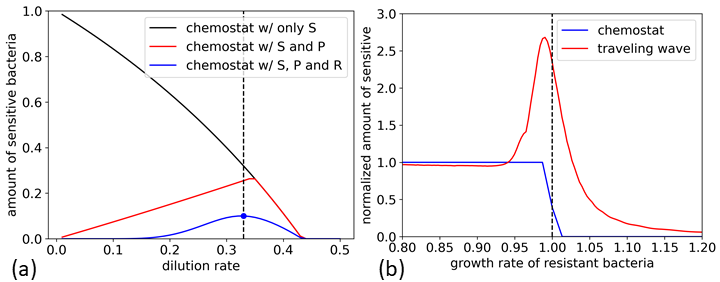
\includegraphics[width=\linewidth]{graphics/2025_09_26_droplets_fig2.png}
\caption{\textbf{Chemostat vs. traveling wave shows protective effect} (a) shows the amount of sensitive bacteria depending on the dilution rate for different scenarios. In black is a scenario with only sensitive bacteria, in red a scenario with phages and sensitive bacteria and in blue a scenario with phages, sensitive and resistant bacteria. (b) shows the normalized amount of sensitive bacteria changing with the growth rate of resistant bacteria for a chemostat (blue) and for a traveling wave (red). The chemostat shows a decrease at the point of equal fitness of resistant and sensitive bacteria. The traveling wave scenario reveals a protective effect resulting in an almost three-fold increase in sensitive bacteria just before the point of equal fitness.}
\label{fig:results_chemostat_traveling_wave}
\end{figure}

\section{Traveling wave dynamics}
Simulating the model with diffusion and initial conditions such that the nutrients are constant and bacteria and phages are concentrated on one side of the system, we obtain a traveling wave dynamics, where bacteria and phages travel together through the system, invading previously unoccupied regions. The nutrients are receding, allowing a sensitive front to be formed. Trailing behind is a phage front which restricts the sensitive bacteria to a narrow region between its front and the phage front. In a narrow intermediate region, a small peak of infected bacteria forms. Resistant bacteria travel uninhibited by phages through the system. These dynamics resemble previously observed experimental results. 

\section{Protection by resistant bacteria}
\label{sec:protective_effect}
Using the established model, we can vary the growth rate of resistant bacteria relative to sensitive bacteria. For low growth rates, we observe survival of sensitive bacteria. For resistant bacteria growth rates higher than the sensitive bacteria growth rate, we see no survival of sensitive bacteria in the system. Surprisingly, for growth rates just below the expected transition point at equal growth rate, we observe a protective effect of the resistant bacteria resulting in an increased amount of sensitive bacteria (Figure~\ref{fig:results_chemostat_traveling_wave}b, red curve). When studying the change of the amount of sensitive bacteria around the maximum over time (Figure~\ref{fig:results_peak_change_height_width}a), we observe a change from a regime where the amount stabilizes quickly and stays constant over a regime where the amount of bacteria constantly linearly increases over time to a regime where after an initial increase, the amount collapses and plateaus or goes towards extinction (Figure~\ref{fig:results_peak_change_height_width}b).

\begin{figure}
\centering
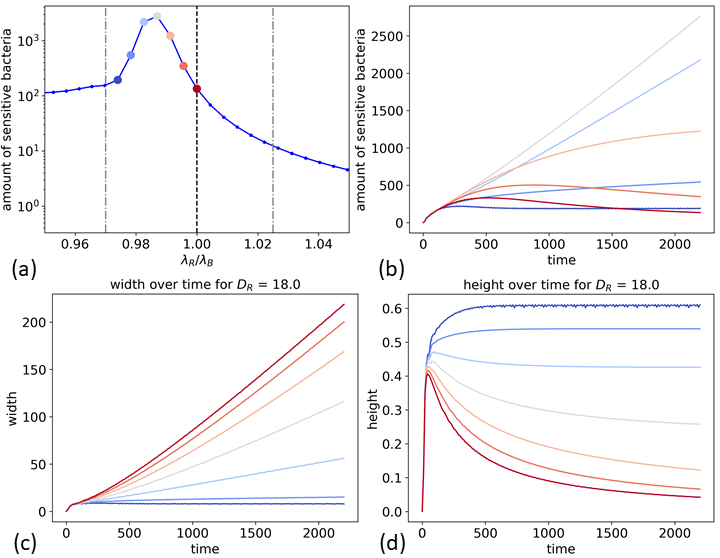
\includegraphics[width=\linewidth]{graphics/2025_09_26_droplets_fig3.png}
\caption{\textbf{Closer examination of the protective peak reveals widening} (a) shows a focused view on the protective peak, described earlier. (b) shows the amount of sensitive bacteria over time for the points indicated with different colors in (a). (c) and (d) show the width and height respectively over time for these chosen points.}
\label{fig:results_peak_change_height_width}
\end{figure}

\section{Widening causes protection}
When studying the width and height of the traveling wave of bacteria, we observe the explanation for the observed protective effect. Monitoring the observed protective peak, we see a transition from a narrow, high peak to a shallow but wide peak of sensitive bacteria with increasing resistant growth rate. Once resistant bacteria grow faster, the sensitive peak disappears. The linear increase in width suggests that the two wave fronts, sensitive bacteria and phages, separated and travel with constant but different speeds. Indeed, measuring the speeds of these two fronts, we observe that the phage front slows down at a lower resistant growth rate than the sensitive bacteria front. However, measuring the difference in speed, we observe that the maximal difference is at a higher growth rate than the observed protective effect. However, as is apparent from our previous height and width analysis, for higher growth rates, the peak is diminished and indeed, multiplying speed with height as a new quantification of the effect, we observe an effect for those growth rates which also reveal the protective effect. So overall, the product of speed difference and height explains the observed protective effect. 
\begin{figure}
\centering
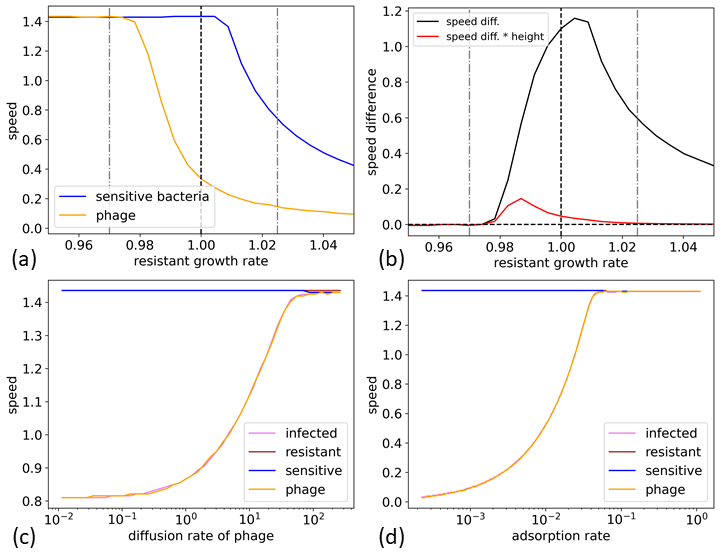
\includegraphics[width=\linewidth]{graphics/2025_09_26_droplets_fig4.png}
\caption{\textbf{Speed difference identified as cause for widening} (a) shows the speed of the expanding wave front of phages and of sensitive bacteria as a function of resistant growth rate, (b) shows the difference between these two speeds and the new measurement of the product between speed difference and height, (c) and (d) show the speed for changing two important parameters, phage diffusion and infection rate respectively.}
\label{fig:results_speed_height}
\end{figure}

\section{Nutrient sparsity weakly protects}
Previous models, studying a phage wave invading an exponentially growing, sensitive population~\cite{Claydon2021-cu} show a separation between the speed of the receding sensitive wave and the speed of the advancing phage wave without resistant bacteria present in the system. Motivated by this results, we are studying in this section, whether we can observe the protective effect in a system without resistant bacteria when instead limiting the available nutrients. Lowering the initially available nutrients in the system, reduces the speed of both waves while for very nutrient concentrations and therefore low speeds a minor speed difference occurs. However, this effect is much smaller than the effect obtained when resistant bacteria are present in the system. Therefore, we conclude that resistant bacteria are necessary to observe the protective effect.
\section{Impact of resistant diffusion rate}
Wave speed and therefore also the bacterial competition are known to not only depend on the growth rate but also on the diffusion rate of the bacteria. Therefore, we analysed the impact changes in both of these parameters on the amount of sensitive bacteria and we found a clear phase transition from a parameter regime in which sensitive bacteria survive to a parameter regime in which sensitive bacteria do not survive~(Figure~\ref{fig:results_heatmap_effect}). Close to the transition interface, we observe the protective effect we previously described in section~\ref{sec:protective_effect}. There seems to be a linear correlation between growth rate and diffusion rate for low growth rates, in agreement with the theoretical results for the KPP-equation. However, for higher growth rates, this linear relation collapses and we observe a dominant effect of growth rate rather than diffusion rate.
\begin{figure}
\centering
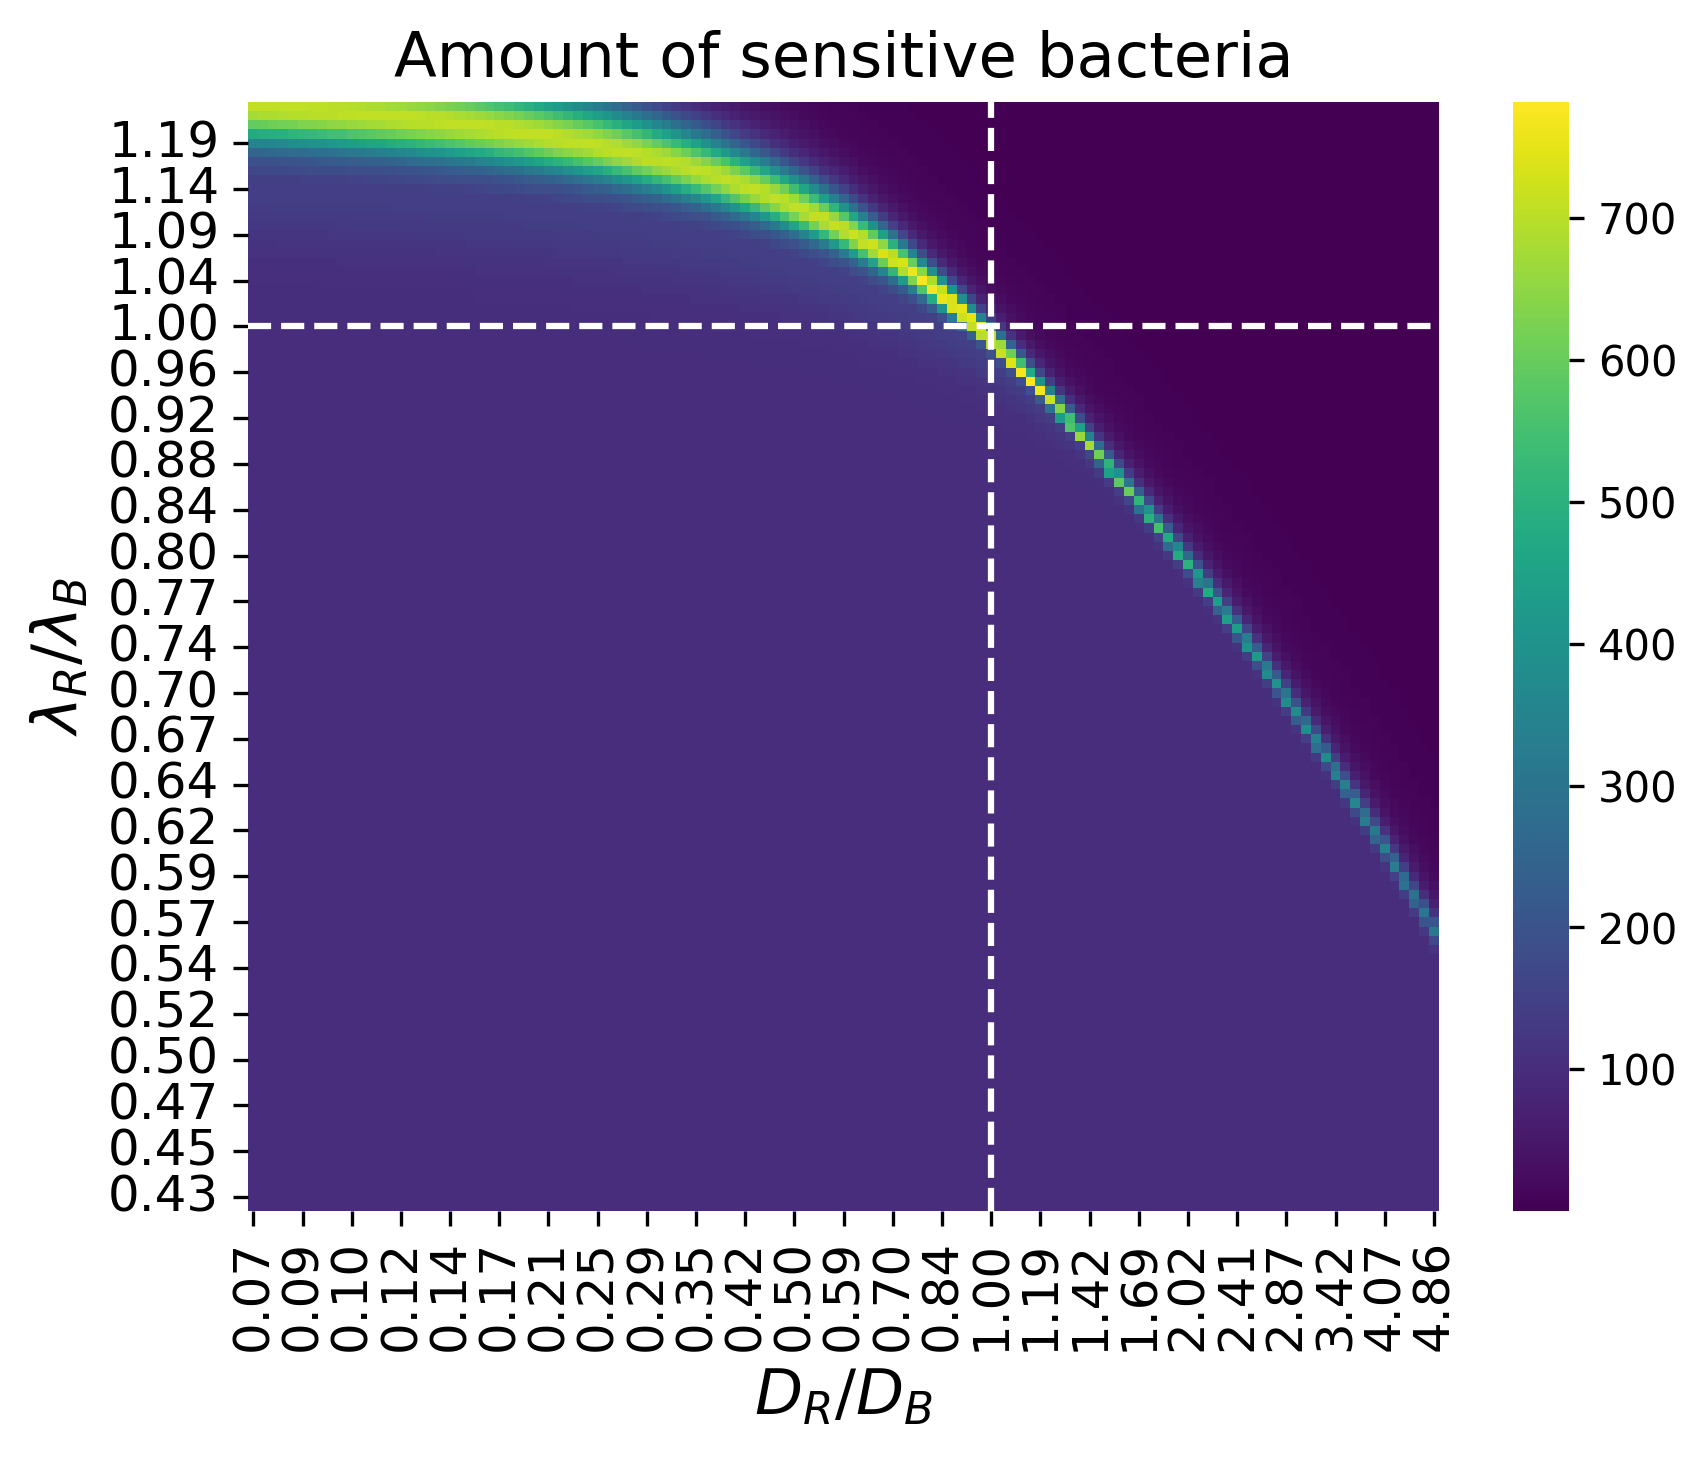
\includegraphics[width=\linewidth]{graphics/2025_09_26_droplets_fig5.png}
\caption{\textbf{Phase transition with two parameters with protective effect} The heatmap shows the amount of sensitive bacteria for different combinations of resistant growth rate and resistant diffusion rate, indicating a phase transition from a region with sensitive bacteria to a region without. At the interface, we observe an increase in sensitive bacteria.}
\label{fig:results_heatmap_effect}
\end{figure}

\section{Impact of parameters}
Our model includes several other parameters, some of which could impact the dynamics. In this section, we are focusing on the phage diffusion rate and the infection rate, both known as parameters whose change can change the phage speed and indeed, we observe that the described protective effect vanishes when phages diffuse faster~(Figure~\ref{fig:results_speed_height}c) or the infection rate is higher~(Figure~\ref{fig:results_speed_height}d). However, while we observe a similar impact of the infection rate in a scenario without resistant bacteria, we do not observe this impact for the phage diffusion rate. 
\section{Limitations}
Some phages replicate only on growing bacteria due to the dependence on the replication machinery of bacteria. Therefore, we explored such a scenario by limiting the infection rate indirectly through a dependence on the nutrients with:
\begin{equation}
    \eta = \eta_0 \frac{n}{K_n + n}
\end{equation}
where $\eta_0$ is set to be the same infection rate as in the scenario without this dependence.
In this scenario, we were unable to observe the protective effect and we rather see a phase transition due to fitness of resistant and sensitive bacteria. Furthermore, if comparing it to a no-phage scenario, where bacteria compete without phages in the system, we see only minor differences between these cases.
This means that the ability for phages to replicate on non-growing bacteria is crucial for the protective effect to exist.

% \chapter{A main chapter}
% \label{chap:firstchap}

% \section{Introduction}

% You might have a per-chapter mini-intro, possibly tying in to the relevant part of the general intro.

% \section{A section}

% \lipsum[1]

% Let's cite a source: \cite{Yao1977}. And now,  let's introduce a (numbered) equation. It will use \gls{symb:c}, which is one of the entries in the ``\nameref{chap:notation-and-abbreviations}'' list. The equation will be in ``display math'' mode, using the \texttt{align} environment.

% \begin{align}
% \label{eq:emc2}
% e &= mc^2
% \end{align}
% \begin{notes}
% \item	Are you seeing a problem with the equation numbering? In some TeX processors and on some platforms, there may be a layout error, so that instead of ``(3.1)'' you get ``)3.1)'' or some other flipping of directions. Specifically, \url{http://overleaf.com} suffers from this problem (at least until 2020). Please make sure and use an appropriate TeX distribution that's up-to-date. Specifically, recent TeXLive versions work fine. On Overleaf, you can switch TeXLive versions using the main menu.
% \end{notes}

% Alternatively, we can use the \texttt{equation} environment with a label. For this to work, our theorem layout package, \texttt{ntheorem}, must be used with the \texttt{amsmath} option. Having done so, let's try our equation:
% \begin{equation}
% \label{eq:power-series}
% f(x)=\sum_{i=0}^{\infty} a_i x^i
% \end{equation}
% Equation \ref{eq:power-series} is a typical power series.

% In \autoref{sec:thm-like} below, we will state some theorems.

% \section{Results... and theorem-like environments}
% \label{sec:thm-like}

% What's so special about the theorem-like environments used here? There are several packages which offer the capability of defining these, mainly \texttt{amsthm}, \texttt{ntheorem} and also \texttt{thmtools}. (The last is probably also the most feature-full and versatile, but I'm not familiar with it and the first two are the popular ones.) Many people writing a Technion thesis start with \texttt{amsthm}, only to find out it has conflicts with Hebrew... also, there's the issue of aliasing (same counter for lemmata and theorems, but having \texttt{{\textbackslash}autoref} and similar commands know what they're referencing.) This is all neatly resolved in \texttt{iitthesis-extra.sty} with \texttt{amsthm}-like-looking environments actually done with nthrerom.

% \begin{theorem}
% \label{thm:first}
% This is the first numbered theorem in this thesis.
% \end{theorem}

% And we can refer to it using \texttt{ref}: \ref{thm:first} and get the number, or use hypertex's \texttt{autoref}: \autoref{thm:first}.

% \begin{corollary}
% \label{cor:first}
% There are no lemmata appearing before theorems in this thesis.
% \end{corollary}

% \begin{theorem*}
% This is the second theorem, unnumbered.
% \end{theorem*}

% \begin{theorem*}[\protect{\cite[Theorem 2]{Knuth1973}}]
% This is an unnumbered theorem cited from elsewhere. \qbfox{1} ... and it was Knuth's dog.
% \end{theorem*}

% \begin{note}
% This is a note environment.  \qbfox{2}
% \end{note}

% \begin{definition}
% \label{def:first}
% An \emph{quick brown fox} is a fox which is not only fast and agile but is also characterized by brown fur. Such foxes sometimes tend to jump over lazy dogs.
% \end{definition}

% \begin{lemma}
% \label{lem:first}
% This is a lemma. \qbfox{2}
% \end{lemma}

% Even though \autoref{lem:first} and \autoref{def:first} share the ``same'' counter, when referring to them, their names are used automagically.

% Here's a proof of the lemma:
% \begin{proof}%[lem:natural:blowups-preserve-distance-on-average]
% \lipsum[2]
% 	It's common to conclude proofs with a QED symbol --- typically a full or an empty black square. To do so, append the command \verb|\qed| after the last sentence of your proof; or, alternatively, you can use some \LaTeX{} trickery in the definition of the proof environment to ensure this symbol is appended to all proofs. This is done in the \texttt{misc/iitthesis-extra.sty} style file, which is used by this template. You will see the result as a black square at the end of this proof environment.
% \end{proof}

% Now here's a proof of \autoref{thm:first} using the \verb|proofof| environment.
% \begin{proofof}[thm:first]
% \lipsum[3]
% \end{proofof}

% \begin{note}There may currently be a problem getting the QED symbol (\verb|\qed|) to appear if your proof environment ends with certain display-mode-math environments, such as \verb|align*|.
% \end{note}

% \begin{proposition}
% \label{prop:first}
% This is a proposition environment. \qbfox{2}
% \end{proposition}

% \begin{observation}
% \label{obs:first}
% The moon revolves around the earth.
% \end{observation}

% There are several other theorem-like environments, of various kinds, defined in the file \texttt{misc/iitthesis-extra.sty}; and naturally you can add or modify these as you see fit.

% \subsection{A subsection}

% We've started a subsection. Here is a reference to another chapter: \autoref{chap:prelims} --- realized with the \verb|\autoref| command. If you've used \texttt{iitthesis-extra.sty}, it should ensure the environment name produced by \verb|\autoref| is capitalized (``Chapter'' rather than ``chapter'').

% \begin{algorithm}
% \caption{A nice algorithm}
% \label{alg:first}
% \begin{algorithmic}[1]
% \FOR{$n$ times}
%   \STATE{Do something.}
%   \STATE{Do something else.}
% \ENDFOR
% \STATE{And do one last thing.}
% \end{algorithmic}
% \end{algorithm}

% It is recommended to use \texttt{algorithmicx} over \texttt{algorithmic} for algorithms, like in \autoref{alg:first}, as it has less conflicts with Hebrew babel (regardless of whether you have Hebrew in your algorithms or not). Also, \texttt{iitthesis-extra.sty} provides it with a necessary workaround.

% \subsection{A second subsection}

% In this subsection we'll have a figure. Remember that the {\LaTeX} compiler can place figures a little before or after where they are defined, according to the placement option choice and depending on the flow of the rest of the text.

% \begin{figure}[htb]
%   \centering
%   \ifpdf
%     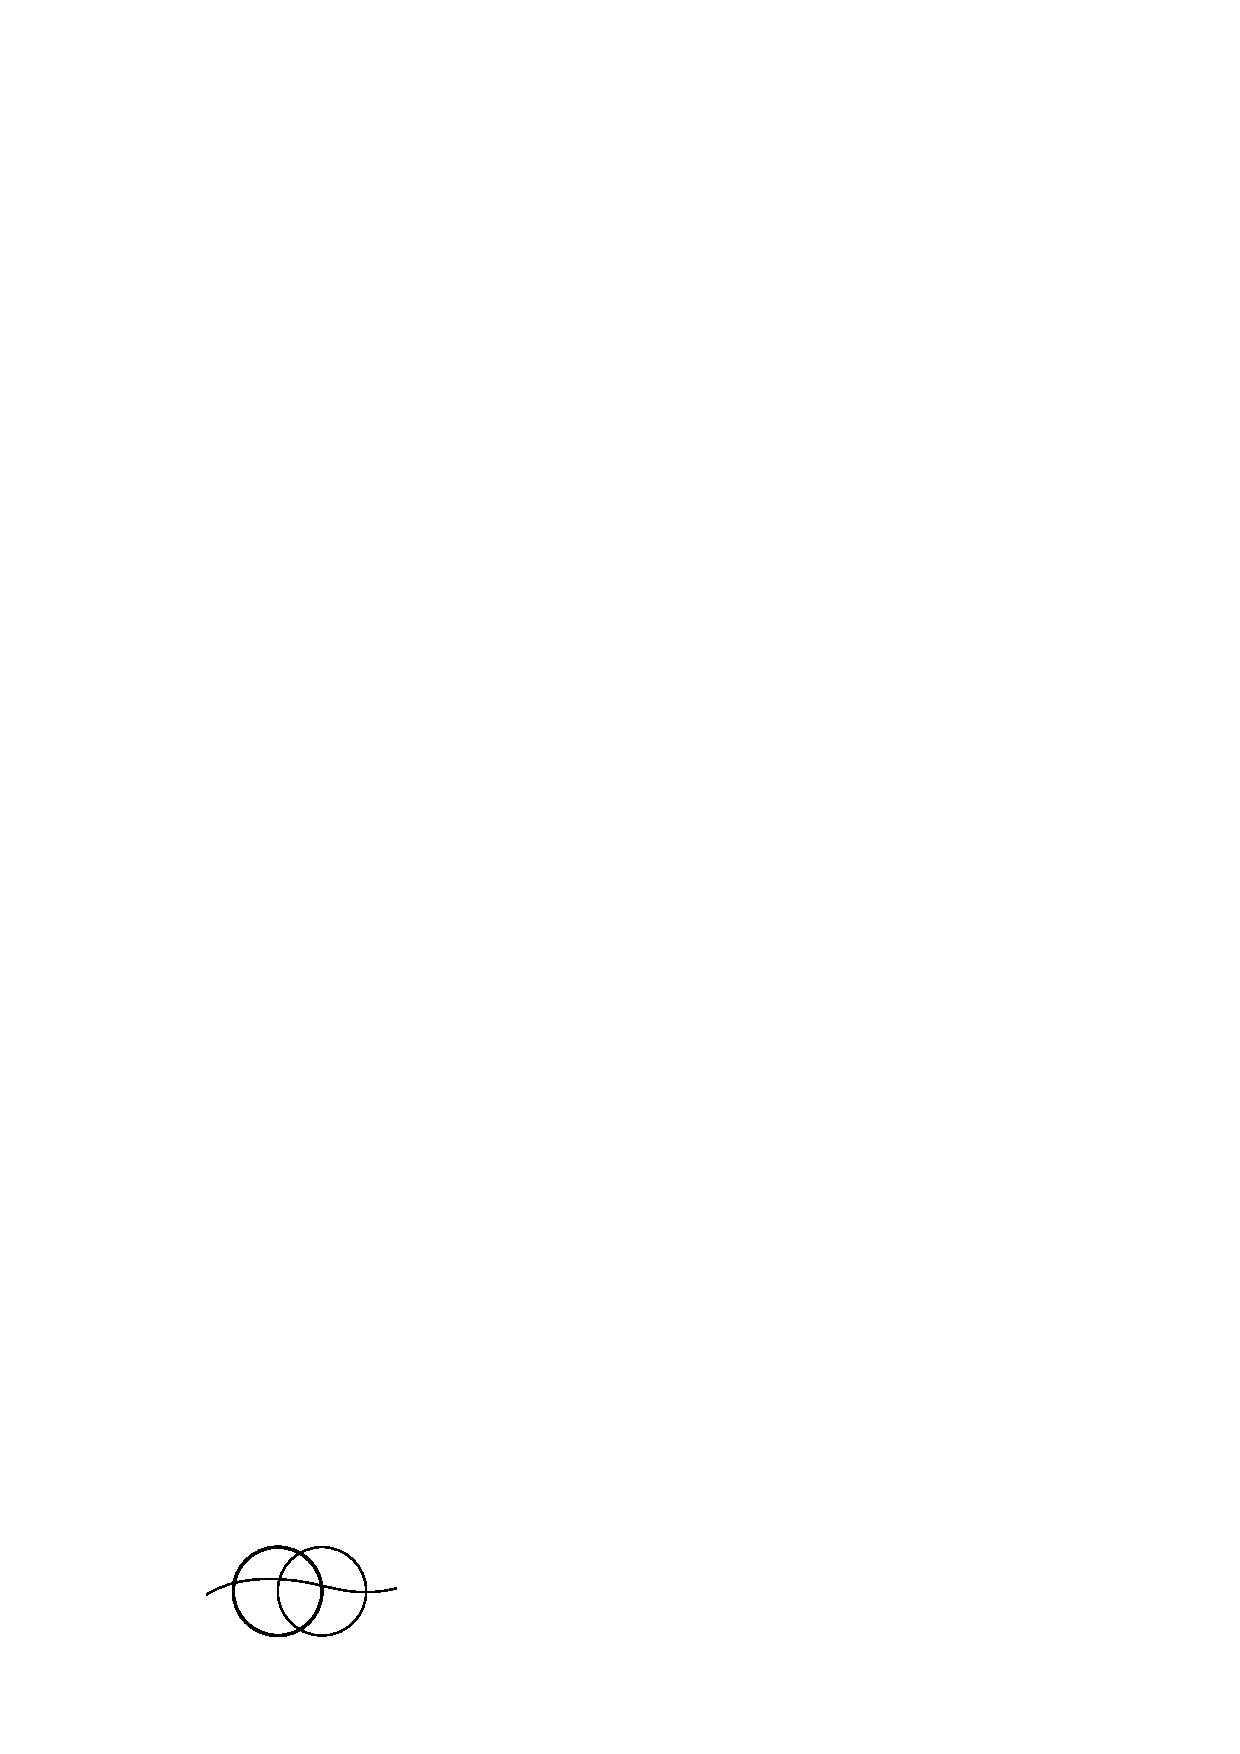
\includegraphics{graphics/mygraphic1.pdf}
%   \else
%     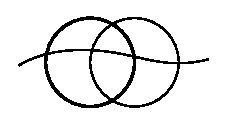
\includegraphics{graphics/mygraphic1-for-ps.eps}
%   \fi
%   \caption{Two circles and a wavy line.}
% \end{figure}

% Let's also have, to conclude this subsection, another use of a term from ``\nameref{chap:notation-and-abbreviations}'', which we first used earlier (in \autoref{chap:prelims}). Here it is: \gls{DIY}. This will ensure it appears on multiple pages; but - its entry will only mention the first appearance, not this one.

\chapter{Conclusion and open questions}
\label{chap:conclusion}

In this project, we built a model to describe bacteria-phage interactions in an expanding traveling wave and studied it in a one-dimensional scenario. We modified the model to allow the study in a zero-dimensional chemostat-like scenario. 
Comparing these two scenarios, our model reveals that in a spatial environment, in complete opposite to a well-mixed environment, adding resistant bacteria to the system can increase the amount of sensitive bacteria in a traveling wave.
Studying the underlying causes for this protective effect, we found that the decoupling of phage and bacterial front causes this protective effect. Through studying different parameter regimes we could determine realistic conditions in which this decoupling and therefore the protective effect is observed.


% This kind of chapter can include may different things (or only some of them):
% \begin{itemize}
% \item Discussion of results
% \item Conclusions from the results or from the process in general
% \item Open questions for future research, resulting from the research performed or from the results obtained
% \end{itemize}

% But not things like the bibliography or other back matter which is generated outside of this chapter.


% \section{Some conclusion}

% Here is what I conclude.

% \section{Some open questions}

% \paragraph{A question in brief.} In \autoref{chap:firstchap} we explored a certain subject, but what about this-or-that idea? Perhaps it is worth exploring. Can one produce interesting results?

% \paragraph{A second question in brief.} A broader exposition of the question and indications of directions or ideas regarding its resolution.


%
% Add any appendices here; they must come _before_ the bibliography
%
\appendix
%\noappendicestocpagenum
%\addappheadtotoc
% \chapter{Some sort of an appendix}
% \label{appendix:somesort}

% You may want to include appendices of your own volition. Also, if you've developed any computer software, that needs to go in as an appendix as well.

% \section{A first section in this appendix}

% Some appendix content here. And something nice to finish things off:

% \begin{figure}[htb]
%   \centering
%   \ifpdf
%     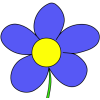
\includegraphics[width=0.3\textwidth]{graphics/mygraphic2.png}
%   \else
%     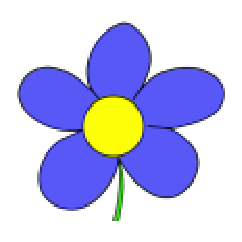
\includegraphics[width=0.3\textwidth]{graphics/mygraphic2-for-ps.eps}
%   \fi
%   \caption{A Flower.}
% \end{figure}

% \section{Another appendix section}
% After the (last) appendix-section comes the thesis' bibliography; Its style is set with the \verb|\thesisbibstyle| command. Then there are the Hebrew parts of thesis, which don't exactly ``follow" the bibliography in a logical sense, but rather start at the beginning of the thesis when considered as a right-to-left printed booklet. Thus, the last page of the extended Hebrew abstract of the thesis comes right ``after" the last page of the bibliography if you're turning the pages in left-to-right order.


% Back Matter
% ------------

% The following command will typeset the bibliography,
% then typeset the Hebrew part of the thesis:
% - Cover page
% - Title page
% - Acknowledgements page
%  (NO table of contents or list of figures in Hebrew)
% - (Extended) abstract (1000-2000 words)
%
% based on information you've provided in the thesis-fields file
% (including the relative paths to your bib files). The Hebrew
% content will be typeset in _reverse_page_order_, i.e. first
% in the file will be the last page of the abstract, and the
% Hebrew cover page will be the last page of the file.
%
\makebackmatter

% The resulting PDF can be printed and taken straight to binding,
% i.e. you do not need to flip any pages anywhere. Of course,
% mind the LaTeX error and warning messages, overfull hboxes etc.

\end{document}

